\documentclass[11pt,a4paper,dvipsnames]{article}
\usepackage[deliverable]{TBCOCoverPage}


\usepackage[margin=2.5cm]{geometry}
\usepackage{tbco}
\usepackage{microtype}
\usepackage{mathpazo} % nice fonts
\usepackage{amsmath}
\usepackage{amssymb}
\usepackage{amsthm}
\usepackage{latexsym}
\usepackage{mathtools}
\usepackage{stmaryrd}
\usepackage{extarrows}
\usepackage{slashed}
\usepackage[colon]{natbib}
\usepackage[unicode=true,pdftex,pdfa,colorlinks=true]{hyperref}
\usepackage{xcolor}
\usepackage[capitalise,noabbrev,nameinlink]{cleveref}
\usepackage{float}
\floatstyle{boxed}
\restylefloat{figure}
\usepackage{tikz}
\usepackage{booktabs}
\usepackage{enumerate}
\usepackage{fancyvrb}
\usepackage{xcolor}


%%
%% Package `semantic` can be used for writing inference rules.
%%
\usepackage{semantic}
%% Setup for the semantic package
\setpremisesspace{20pt}

% data for Deliverable header -- added by KH from an EU H2020 project template
\DeliverableNumber{GL-D1}
\DeliverableTitle{A Formal Specification of the Bcc Ledger with a Native Multi-Asset Implementation}
   {Formal Bcc Ledger with Multi-Asset Spec.}

\DeliverableResponsible{Formal Methods Team}

\DueDate{31$^{\textrm{st}}$ July 2020}

\SubmissionDate{20$^{\textrm{st}}$ August 2020}{20$^{\textrm{st}}$ August 2020}

\Authors{
   Polina Vinogradova \quad \texttt{polina.vinogradova@tbco.io} \\
   Andre Knispel \quad \texttt{andre.knispel@tbco.io}
}

\EditorName{Polina Vinogradova}
\LeaderName{Philipp Kant, \TBCO}
\InstitutionAddress{\TBCO}
\Version{1.0}
\Project{Charles Ledger}
\DisseminationPU

%%
%% Types
%%
\newcommand{\Nothing}{\ensuremath{\Diamond}}
\newcommand{\N}{\ensuremath{\mathbb{N}}}
\newcommand{\Bool}{\type{Bool}}
\newcommand{\Npos}{\ensuremath{\mathbb{N}^{+}}}
\newcommand{\Z}{\ensuremath{\mathbb{Z}}}
\newcommand{\R}{\ensuremath{\mathbb{R}}}
\newcommand{\Rnn}{\ensuremath{\mathbb{R}^{\geq 0}}}
\newcommand{\Tx}{\type{Tx}}
\newcommand{\SophieTx}{\type{SophieTx}}
\newcommand{\CharlesTx}{\type{CharlesTx}}
\newcommand{\TxBody}{\type{TxBody}}
\newcommand{\UnsignedData}{\type{UnsignedData}}
\newcommand{\VldSR}{\type{VldSR}}
\newcommand{\VldOut}{\type{VldOut}}
\newcommand{\Vlds}{\type{Vlds}}
\newcommand{\TxWitness}{\type{TxWitness}}
\newcommand{\Ix}{\type{Ix}}
\newcommand{\RdmrPtr}{\type{RdmrPtr}}
\newcommand{\TxId}{\type{TxId}}
\newcommand{\Addr}{\type{Addr}}
\newcommand{\UTxO}{\type{UTxO}}
\newcommand{\UTxOIn}{\type{UTxOIn}}
\newcommand{\UTxOOut}{\type{UTxOOut}}
\newcommand{\Wdrl}{\type{Wdrl}}
\newcommand{\Coin}{\type{Coin}}
\newcommand{\PParams}{\type{PParams}}
\newcommand{\SophiePParams}{\type{SophiePParams}}
\newcommand{\NewParams}{\type{NewParams}}
\newcommand{\Slot}{\type{Slot}}
\newcommand{\SlotsPrior}{\ensuremath{\mathsf{SlotsPrior}}}
\newcommand{\SlotsPerEpoch}{\mathsf{SlotsPerEpoch}}
\newcommand{\SlotsPerKESPeriod}{\mathsf{SlotsPerKESPeriod}}
\newcommand{\SlotsStabilityParam}{\fun{k}}
\newcommand{\Duration}{\type{Duration}}
\newcommand{\StakePools}{\type{StakePools}}
\newcommand{\StakeDeleg}{\type{StakeDeleg}}
\newcommand{\StakeCreds}{\type{StakeCreds}}
\newcommand{\Seed}{\type{Seed}}
\newcommand{\seedOp}{\star}
\newcommand{\Ppm}{\type{Ppm}}
\newcommand{\Value}{\type{Value}}
\newcommand{\ProtVer}{\ensuremath{\type{ProtVer}}}
\newcommand{\Language}{\type{Language}}
\newcommand{\ApName}{\ensuremath{\type{ApName}}}
\newcommand{\ApVer}{\ensuremath{\type{ApVer}}}
\newcommand{\SystemTag}{\ensuremath{\type{SystemTag}}}
\newcommand{\InstallerHash}{\ensuremath{\type{InstallerHash}}}
\newcommand{\PPUpdate}{\type{PPUpdate}}
\newcommand{\Applications}{\type{Applications}}
\newcommand{\AVUpdate}{\type{AVUpdate}}
\newcommand{\Update}{\type{Update}}
\newcommand{\DCert}{\type{DCert}}
\newcommand{\DCertRegKey}{\type{DCert_{regkey}}}
\newcommand{\DCertDeRegKey}{\type{DCert_{deregkey}}}
\newcommand{\DCertDeleg}{\type{DCert_{delegate}}}
\newcommand{\DCertRegPool}{\type{DCert_{regpool}}}
\newcommand{\DCertRetirePool}{\type{DCert_{retirepool}}}
\newcommand{\DCertGen}{\type{DCert_{genesis}}}
\newcommand{\DCertMir}{\type{DCert_{mir}}}
\newcommand{\PoolParam}{\type{PoolParam}}
\newcommand{\UTxOState}{\ensuremath{\type{UTxOState}}}
\newcommand{\SFState}{\ensuremath{\type{SFState}}}
\newcommand{\ledgerState}{\ensuremath{\type{ledgerState}}}
\newcommand{\ValEnv}{\type{ValEnv}}
\newcommand{\ValState}{\type{ValState}}
\newcommand{\ScrInData}{\type{ScrInData}}
\newcommand{\AddrRWD}{\type{Addr_{rwd}}}
\newcommand{\AddrB}{\type{Addr_{base}}}
\newcommand{\AddrP}{\type{Addr_{ptr}}}
\newcommand{\AddrE}{\type{Addr_{enterprise}}}
\newcommand{\AddrBS}{\type{Addr_{bootstrap}}}
\newcommand{\Ptr}{\type{Ptr}}
\newcommand{\DState}{\type{DState}}
\newcommand{\DWEnv}{\type{DWEnv}}
\newcommand{\DPSEnv}{\type{DPSEnv}}
\newcommand{\DPEnv}{\type{DPEnv}}
\newcommand{\DEnv}{\type{DEnv}}
\newcommand{\PEnv}{\type{PEnv}}
\newcommand{\DPState}{\type{DPState}}
\newcommand{\PState}{\type{PState}}
\newcommand{\DCertBody}{\type{DCertBody}}
\newcommand{\TData}{\type{TData}}
\newcommand{\DPoolReap}{\ensuremath{\type{poolreap}}}
\newcommand{\UPIState}{\type{UPIState}}
\newcommand{\UpdatePayload}{\type{UpdatePayload}}
\newcommand{\NetworkId}{\mathsf{NetworkId}}
\newcommand{\MemoryEstimate}{\type{MemoryEstimate}}

% multi-signature
\newcommand{\StakeCredential}{\type{Credential}_{stake}}
\newcommand{\StakeDelegs}{\type{StakeDelegs}}
\newcommand{\Quorum}{\type{Quorum}}

\newcommand{\txwitsVKey}[1]{\fun{txwitsVKey}~\var{#1}}
\newcommand{\txwitsScript}[1]{\fun{txwitsScript}~\var{#1}}

\newcommand{\AddrVKey}{\type{Addr^{vkey}}}
\newcommand{\AddrRWDVKey}{\type{Addr_{rwd}^{vkey}}}
\newcommand{\AddrRWDScr}{\type{Addr_{rwd}^{script}}}
\newcommand{\AddrVKeyB}{\type{Addr^{vkey}_{base}}}
\newcommand{\AddrVKeyP}{\type{Addr^{vkey}_{ptr}}}
\newcommand{\AddrVKeyE}{\type{Addr^{vkey}_{enterprise}}}
\newcommand{\AddrVKeyBS}{\type{Addr^{vkey}_{bootstrap}}}
\newcommand{\AddrScr}{\type{Addr^{script}}}
\newcommand{\AddrScrBase}{\type{Addr_{base}^{script}}}
\newcommand{\AddrScrEnterprise}{\type{Addr_{enterprise}^{script}}}
\newcommand{\AddrScrPtr}{\type{Addr_{ptr}^{script}}}
\newcommand{\AuxiliaryData}{\type{AuxiliaryData}}
\newcommand{\AuxiliaryDataHash}{\type{AuxiliaryDataHash}}
\newcommand{\Metadata}{\type{Metadata}}
\newcommand{\DataHash}{\type{DataHash}}
\newcommand{\ScriptHash}{\type{ScriptHash}}
\newcommand{\PolicyID}{\type{PolicyID}}
\newcommand{\PPHash}{\type{PPHash}}
\newcommand{\RdmrsHash}{\type{RdmrsHash}}
\newcommand{\Script}{\type{Script}}
\newcommand{\ScriptZerepoch}{\type{Script}_{plc}}
\newcommand{\ScriptNI}{\type{Script^{native}_{v1}}}
\newcommand{\Timelock}{\type{Script^{native}_{v2}}}
\newcommand{\ScriptMSig}{\type{Script}_{msig}}
\newcommand{\ScriptV}{\type{Script_{v}}}
\newcommand{\Datum}{\type{Datum}}
\newcommand{\Rdmr}{\type{Rdmr}}
\newcommand{\CurItem}{\type{CurItem}}
\newcommand{\Rdmrs}{\type{Rdmrs}}
\newcommand{\DorR}{\type{DorR}}
\newcommand{\ValidationData}{\type{ValidationData}}
\newcommand{\IsValidating}{\type{IsValidating}}
\newcommand{\HashUnsData}{\type{HashUnsData}}
\newcommand{\True}{\type{True}}
\newcommand{\False}{\type{False}}
\newcommand{\MSig}{\type{MSig}}
\newcommand{\Credential}{\type{Credential}}
\newcommand{\AssetID}{\type{AssetID}}
\newcommand{\AssetName}{\type{AssetName}}
\newcommand{\Quantity}{\type{Quantity}}
\newcommand{\QuantityPM}{\type{Quantity}^{\pm}}
\newcommand{\ValuePM}{\type{Value}^{\pm}}

%% Adding witnesses
\newcommand{\TxIn}{\type{TxIn}}
\newcommand{\OutRef}{\type{OutRef}}
\newcommand{\SophieTxIn}{\type{SophieTxIn}}
\newcommand{\SophieTxOut}{\type{SophieTxOut}}
\newcommand{\SophieUTxO}{\type{SophieUTxO}}
\newcommand{\SophieChainState}{\type{SophieChainState}}
\newcommand{\HasDV}{\type{HasDV}}
\newcommand{\TxInScr}{\type{TxInScr}}
\newcommand{\Info}{\type{Info}}
\newcommand{\ExUnits}{\type{ExUnits}}
\newcommand{\CostMod}{\type{CostMod}}
\newcommand{\Prices}{\type{Prices}}
\newcommand{\IsFee}{\type{IsFee}}
\newcommand{\TxOut}{\type{TxOut}}
\newcommand{\OutFoo}{\type{OutFoo}}
\newcommand{\TxOutND}{\type{TxOutND}}
\newcommand{\TxOutP}{\type{TxOutP}}
\newcommand{\VKey}{\type{VKey}}
\newcommand{\VKeyEv}{\type{VKey_{ev}}}
\newcommand{\VKeyGen}{\type{VKey_G}}
\newcommand{\SKey}{\type{SKey}}
\newcommand{\SKeyEv}{\type{SKey_{ev}}}
\newcommand{\KeyHash}{\type{KeyHash}}
\newcommand{\KeyHashGen}{\type{KeyHash_G}}
\newcommand{\KeyPair}{\type{KeyPair}}
\newcommand{\KeyPairEv}{\type{KeyPair_{ev}}}
\newcommand{\Sig}{\type{Sig}}
\newcommand{\Data}{\type{Data}}
%% Adding delegation
\newcommand{\Epoch}{\type{Epoch}}
\newcommand{\KESPeriod}{\type{KESPeriod}}
%% Blockchain
\newcommand{\Gkeys}{\var{G_{keys}}}
\newcommand{\Block}{\type{Block}}
\newcommand{\SlotId}{\type{SlotId}}
\newcommand{\PPUpdateEnv}{\type{PPUpdateEnv}}
\newcommand{\AVUpdateEnv}{\type{AVUpdateEnv}}
\newcommand{\AVUpdateState}{\type{AVUpdateState}}
\newcommand{\UpdateEnv}{\type{UpdateEnv}}
\newcommand{\UpdateState}{\type{UpdateState}}
\newcommand{\UTxOEnv}{\type{UTxOEnv}}
\newcommand{\CEEnv}{\type{CEEnv}}
\newcommand{\CEState}{\type{CEState}}
\newcommand{\BDEnv}{\type{BDEnv}}
\newcommand{\BDState}{\type{BDState}}
\newcommand{\LEnv}{\type{LEnv}}
\newcommand{\LState}{\type{LState}}
\newcommand{\CharlesChainState}{\type{CharlesChainState}}
%%
%% Functions
%%
\newcommand{\txins}[1]{\fun{txins}~ \var{#1}}
\newcommand{\txouts}[1]{\fun{txouts}~ \var{#1}}
\newcommand{\txcerts}[1]{\fun{txcerts}~ \var{#1}}
\newcommand{\txid}[1]{\fun{txid}~ \var{#1}}
\newcommand{\outs}[1]{\fun{outs}~ \var{#1}}
\newcommand{\values}[1]{\fun{values}~ #1}
\newcommand{\ubalance}[1]{\fun{ubalance}~ \var{#1}}
\newcommand{\txttl}[1]{\fun{txttl}~ \var{#1}}
\newcommand{\firstSlot}[1]{\fun{firstSlot}~ \var{#1}}
\newcommand{\totalDeposits}[3]{\fun{totalDeposits}~ \var{#1} ~ \var{#2} ~ \var{#3}}
\newcommand{\decayedKey}[4]{\fun{decayedKey}~ \var{#1}~ \var{#2}~ \var{#3}~ \var{#4}}
\newcommand{\decayedTx}[3]{\fun{decayedTx}~ \var{#1}~ \var{#2}~ \var{#3}}
\newcommand{\keyRefund}[6]{\fun{keyRefund}~ {#1}~{#2}~{#3}~\var{#4}~\var{#5}~\var{#6}}
\newcommand{\refund}[4]{\fun{refund}~ \var{#1}~ \var{#2}~ {#3}~ {#4}}
\newcommand{\keyRefunds}[2]{\fun{keyRefunds}~ \var{#1}~ \var{#2}}
\newcommand{\consumed}[2]{\fun{consumed}~ \var{#1}~ \var{#2}}
\newcommand{\produced}[2]{\fun{produced}~ \var{#1}~ \var{#2}}
\newcommand{\applyFun}[2]{\fun{#1}~\var{#2}}

\newcommand{\RegKey}[1]{\textsc{RegKey}(#1)}
\newcommand{\DeregKey}[1]{\textsc{DeregKey}(#1)}
\newcommand{\Delegate}[1]{\textsc{Delegate}(#1)}
\newcommand{\RegPool}[1]{\textsc{RegPool}(#1)}
\newcommand{\RetirePool}[1]{\textsc{RetirePool}(#1)}
\newcommand{\cwitness}[1]{\fun{cwitness}~ \var{#1}}
\newcommand{\dpool}[1]{\fun{dpool}~ \var{#1}}
\newcommand{\poolParam}[1]{\fun{poolParam}~ \var{#1}}
\newcommand{\retire}[1]{\fun{retire}~ \var{#1}}
\newcommand{\addrRw}[1]{\fun{addr_{rwd}}~ \var{#1}}
\newcommand{\epoch}[1]{\fun{epoch}~\var{#1}}
\newcommand{\kesPeriod}[1]{\fun{kesPeriod}~\var{#1}}

%% UTxO witnesses
\newcommand{\inputs}[1]{\fun{inputs}~ \var{#1}}
\newcommand{\txwits}[1]{\fun{txwits}~ \var{#1}}
\newcommand{\verify}[3]{\fun{verify} ~ #1 ~ #2 ~ #3}
\newcommand{\sign}[2]{\fun{sign} ~ #1 ~ #2}
\newcommand{\verifyEv}[4]{\fun{verify_{ev}} ~ #1 ~ #2 ~ #3 ~ #4}
\newcommand{\signEv}[3]{\fun{sign_{ev}} ~ #1 ~ #2 ~ #3}
\newcommand{\serialised}[1]{\llbracket \var{#1} \rrbracket}
\newcommand{\hashKey}[1]{\fun{hashKey}~ \var{#1}}
\newcommand{\txbody}[1]{\fun{txbody}~ \var{#1}}
\newcommand{\txfee}[1]{\fun{txfee}~ \var{#1}}
\newcommand{\txwdrls}[1]{\fun{txwdrls}~ \var{#1}}
\newcommand{\minfee}[2]{\fun{minfee}~ \var{#1}~ \var{#2}}
\newcommand{\slotminus}[2]{\var{#1}~-_{s}~\var{#2}}
\DeclarePairedDelimiter\floor{\lfloor}{\rfloor}
% wildcard parameter
\newcommand{\wcard}[0]{\underline{\phantom{a}}}
%% Adding ledgers...
\newcommand{\utxo}[1]{\fun{utxo}~ #1}
%% Delegation
\newcommand{\delegatesName}{\fun{delegates}}
\newcommand{\delegates}[3]{\delegatesName~#1~#2~#3}
\newcommand{\dwho}[1]{\fun{dwho}~\var{#1}}
\newcommand{\depoch}[1]{\fun{depoch}~\var{#1}}
\newcommand{\dval}{\ensuremath{d_{\mathsf{val}}}}
%% Delegation witnesses
\newcommand{\dbody}[1]{\fun{dbody}~\var{#1}}
\newcommand{\dwit}[1]{\fun{dwit}~\var{#1}}
%% Blockchain
\newcommand{\bwit}[1]{\fun{bwit}~\var{#1}}
\newcommand{\bslot}[1]{\fun{bslot}~\var{#1}}
\newcommand{\bbody}[1]{\fun{bbody}~\var{#1}}
\newcommand{\bhbody}[1]{\fun{bhbody}~\var{#1}}
\newcommand{\bdlgs}[1]{\fun{bdlgs}~\var{#1}}
%% ledgerstate constants
\newcommand{\genesisId}{\ensuremath{Genesis_{Id}}}
\newcommand{\genesisTxOut}{\ensuremath{Genesis_{Out}}}
\newcommand{\genesisUTxO}{\ensuremath{Genesis_{UTxO}}}
\newcommand{\genesisUTxOState}{(\genesisUTxO,\wcard,\wcard,\wcard)}
\newcommand{\emax}{\ensuremath{\mathsf{E_{max}}}}

\newcommand{\unitInterval}{\ensuremath{[0,~1]}}
\newcommand{\unitIntervalNonNull}{\ensuremath{(0,~1]}}
\newcommand{\nonnegReals}{\ensuremath{[0,~\infty)}}
\newcommand{\posReals}{\ensuremath{(0,~\infty)}}

\theoremstyle{definition}
\newtheorem{definition}{Definition}[section]
\newtheorem{lemma}[definition]{Lemma}
\newtheorem{theorem}[definition]{Theorem}
\newtheorem{property}{Property}[section]

\newcommand{\leteq}{\ensuremath{\mathrel{\mathop:}=}}

\newcommand{\arrow}{\rightarrow}

\definecolor{hldiffcolor}{rgb}{0.95, 0.93, 0}
\newcommand{\hldiff}[1]{\mathchoice
  {\colorbox{hldiffcolor}{$\displaystyle#1$}}
  {\colorbox{hldiffcolor}{$\textstyle#1$}}
  {\colorbox{hldiffcolor}{$\scriptstyle#1$}}
  {\colorbox{hldiffcolor}{$\scriptscriptstyle#1$}}}
\DeclareMathOperator{\supp}{supp}

\newcommand{\khcomment}[1]{\textbf{ -- KH: #1 -- }}
\renewcommand{\khcomment}[1]{} % For publication

\begin{document}

\hypersetup{
  pdftitle={A Formal Specification of the Bcc Ledger},
  breaklinks=true,
  bookmarks=true,
  colorlinks=false,
  linkcolor={blue},
  citecolor={blue},
  urlcolor={blue},
  linkbordercolor={white},
  citebordercolor={white},
  urlbordercolor={white}
}

  \cleardoublepage%
  \tableofcontents%

  \listoffigures%
  \clearpage%

  \begin{changelog}
        \change{2019/10/08}{Jared Corduan, Polina Vinogradova and Matthias G\"udemann}{FM (TBCO)}{Initial version (0.1).}
        \change{2019/10/08}{Kevin Hammond}{FM (TBCO)}{Added cover page.}
        \change{2020/11/17}{Jared Corduan}{FM (TBCO)}
          {Removed unused deliverable outline image,
           set version to 1.0,
           and changed the reward calculation so that $\eta$
             takes $d$ into account.}
        \change{2021/05/17}{Jared Corduan}{FM (TBCO)}{Added Example Illustration.}
        \change{2021/06/14}{Jared Corduan}{FM (TBCO)}
          {Added an errata section,
           fixed a typo in leader check and in the LEDGERS rule index,
           and synced the reward calculation with the implementation}
        \change{2021/06/17}{Jared Corduan}{FM (TBCO)}
          {Allow the pool influence parameter $a_0$ to be zero,
          remove all mentions of deposit decay, sync varibale names with code.}
        \change{2021/08/27}{Jared Corduan}{FM (TBCO)}{Fixed definitions in the header-only validation properties.
          CHAIN transition did not need to use previous protocol parameters.}
      \end{changelog}
      \clearpage%
\renewcommand{\thepage}{\arabic{page}}
\setcounter{page}{1}

\title{A Formal Specification of the Bcc Ledger}

\author{Jared Corduan  \\ {\small \texttt{jared.corduan@tbco.io}} \\
   \and Polina Vinogradova \\ {\small \texttt{polina.vinogradova@tbco.io}} \\
   \and Matthias G\"udemann  \\ {\small \texttt{matthias.gudemann@tbco.io}}}

%\date{}

\maketitle

\begin{abstract}
This document provides a formal specification of the Bcc ledger for use in the upcoming Sophie implementation.
It is intended to underpin a Haskell executable specification that will be the basis of the initial
Sophie release, and represents a core design and quality assurance document.
It will be used to define properties and tests, and to provide the basis for strong formal assurance
using mathematical proof techniques.
The document defines the rules for extending the ledger with transactions
that will affect both UTxO and stake delegation.
Key properties that have been identified include the preservation of balances, absence of double spend, stakepool registration,
and reward splitting.
\end{abstract}

\section*{List of Contributors}
\label{acknowledgements}

Nicol\'as Arqueros,
Nicholas Clarke,
Duncan Coutts,
Ruslan Dudin,
Sebastien Guillemot,
Kevin Hammond,
Vincent Hanquez,
Ru Horlick,
Michael Hueschen,
Yun Lu,
Philipp Kant,
Jean-Christophe Mincke,
Damian Nadales,
Ashish Prajapati,
Nicolas Di Prima,
Andrew Westberg.


\pagebreak
\tableofcontents
\listoffigures

\section{Introduction}

The focus of this document is to give a description of the changes
required to support multi-assets on the Sophie ledger as described in
\cite{utxo_ma}. These multi-assets are implemented via token bundles,
given by a type called $\Value$, which replace the type $\Coin$ of the
Sophie ledger in many (but not all) cases.

All aspects of the ledger not given in this document are as specified
in the Sophie ledger design and implementation~\cite{sophie_spec},
but if they depend on something that is changed in this version of the
ledger they must use the definitions from this document.

\section{Notation}

In addition to the notation in the Sophie spec, we use the following notations:

\begin{description}
\item[Functions with finite support] For a monoid $M$, $A \to_0 M$
  are the functions $f : A \to M$ with finite support, i.e. such that
  there exist only finitely many $a \in A$ such that $f a \neq 0$. We
  denote the support of $f$ by $\supp f$, which is defined as
  $\supp f := \{ a \in A : f a \neq 0 \}$.
\end{description}

\section{Coin and Multi-Asset Tokens}
\label{sec:coin-ma}

This section describes the type $\Value$, the operations required on
it, and its relation to $\Coin$.

When multi-asset support on the ledger is introduced, Bcc is still expected to be
the most common type of token on the ledger.
The $\Coin$ type is used to represent an amount of Bcc.
It is the only
type of token that can be used for all non-UTxO ledger accounting, including deposits,
fees, rewards, treasury, and the proof of stake protocol.

\begin{figure*}[t!]
  \emph{Abstract Types}
  %
  \begin{align*}
    \var{aname} \in& ~\AssetName & \text{Asset Names}
  \end{align*}
  %
  \emph{Derived types}
  %
  \begin{equation*}
    \begin{array}{r@{~\in~}l@{\qquad=\qquad}lr}
      \var{pid} & \PolicyID & \ScriptHash \\
      \var{quan} & \Quantity & \Z \\
      %\text{quantity of a token}\\
      \var{v}, \var{w} & \Value
      & \PolicyID \to_0 ( \AssetName \to_0 \Quantity )
%      & \text{a collection of tokens}
    \end{array}
  \end{equation*}
  %
  \emph{Abstract Functions and Values}
  %
  \begin{align*}
    \mathsf{bccPolicy} \in& ~\PolicyID & \text{Bcc Policy ID} \\
    \mathsf{bccName} \in& ~\AssetName & \text{Bcc Asset Name} \\
    \mathsf{size} \in& ~\Value\to\MemoryEstimate & \text{the size of a Value}
  \end{align*}
  \emph{Helper Functions}
  %
  \begin{align*}
    & \fun{inject} \in \Coin\to \Value \\
    & \fun{inject}~c = \lambda~\var{pid}~\var{aname}.
      \begin{cases}
        c & \var{pid} = \mathsf{bccPolicy}~\text{and}~\var{aname} = \mathsf{bccName} \\
        0 & \text{otherwise}
      \end{cases}
    \nextdef
    & \fun{coin} \in \Value \to \Coin \\
    & \fun{coin}~v = v~\mathsf{bccPolicy}~\mathsf{bccName}
    \nextdef \fun{inject} \circ \fun{coin}
    & \fun{bccOnly} \in \Value \to \Bool \\
    & \fun{bccOnly}~v =
      \begin{cases}
        \True & \fun{inject} \circ \fun{coin} = \fun{id}_{\Value} \\
        \False & \text{otherwise}
      \end{cases}
  \end{align*}
  \caption{Type Definitions and auxiliary functions for Value}
  \label{fig:defs:value}
\end{figure*}

\subsection*{Representing Multi-asset Types and Values}
We will refer to a pair of a $\PolicyID$ and an
$\AssetName$ as an $\AssetID$. The $\AssetID$ for Bcc is $(\mathsf{bccPolicy}, \mathsf{bccName})$.
This is symbolic only, no actual minting policy for Bcc exists.

The set of tokens that are referred to by the underlying monetary
policy represents the coinage that the asset supports. A multi-asset
value, $\Value$ is a finitely supported function of two variables,
$\PolicyID$ and $\AssetName$ to $\Quantity$.

\begin{itemize}
  \item $\PolicyID$ identifies monetary policies. A policy ID $\var{pid}$ is associated with a script
    $s$ such that $\fun{hashScript}~s~=~pid$. When a transaction attempts to create or destroy tokens
    that fall under the policy ID $\var{pid}$,
    $s$ verifies that the transaction
    respects the restrictions that are imposed by the monetary policy.
    See sections \ref{sec:transactions} and \ref{sec:utxo} for details.

  \item $\AssetName$ is a type used to distinguish different tokens with the same $\PolicyID$.
    Each $aname$ identifies a unique kind of token in $\var{pid}$.

  \item $\Quantity$ is an integer type that represents an amount of a specific $\AssetName$. We associate
    a term $q\in\Quantity$ with a specific token to track how much of that token is contained in a given asset value.

  \item $\Value$ is the multi-asset type that is used to represent
    a collection of tokens, including Bcc. If $(\var{pid}, \var{aname})$ is an $\AssetID$ and $v \in \Value$,
    the quantity in $v$ belonging to that $\AssetID$ is $v~\var{pid}~\var{aname}$.
    Tokens are fungible with each other if and only if they belong to the same $\AssetID$,
    i.e. they have the same $\PolicyID$ and $\AssetName$. Terms of type $\Value$ are sometimes also referred to as
    \emph{token bundles}.

  \item $\mathsf{bccPolicy}$ and $\mathsf{bccName}$ are the $\PolicyID$ and $\AssetName$ of Bcc respectively.
    It is not possible to mint any token with the $\PolicyID$ $\mathsf{bccPolicy}$, which means that every
    token in the UTxO belonging to $\mathsf{bccPolicy}$ will have $\AssetName$ $\mathsf{bccName}$.

  \item $\mathsf{size}$ returns the size (in units of memory, eg. bytes or words) of a $\Value$.
  We give this function, alongside implementation-specific constants we have used in it in Section \ref{sec:value-size}.

  \item $\fun{inject}$ and $\fun{coin}$ convert between the two types,
  by building a $\Value$ that only contains Bcc given by the input, and extracting
  the amount of Bcc as (a $\Coin$) from a $\Value$ respectively.
  Note that composed as

  \[\fun{coin} \circ \fun{inject} = \fun{id}_{\Coin}\]

  these functions give the identity on $\Coin$, but composed in the opposite order as

  \[\fun{inject} \circ \fun{coin}\]

  they return a $\Value$ containing only the Bcc tokens contained in the original $\Value$.

  \item $\fun{bccOnly}$ returns $\True$ if a given $\Value$ contains only Bcc.
\end{itemize}

\subsection*{Value Operations and Partial Order}
We require some operations on $\Value$, including equality, addition and $\leq$ comparison.

Addition and binary relations are extended pointwise from $\Coin$ to $\Value$, so if $R$ is a binary relation defined on $\Coin$, like $=$ or $\leq$, and $v, w$ are values, we define

\[ v~R~w :\Leftrightarrow \forall~\var{pid}~\var{aname}, (v~\var{pid}~\var{aname})~R~(w~\var{pid}~\var{aname}) \]
\[ (v + w)~\var{pid}~\var{aname} := (v~\var{pid}~\var{aname}) + (w~\var{pid}~\var{aname}). \]

\section{Transactions}
\label{sec:transactions}

Transactions are defined in Figure~\ref{fig:defs:utxo-sophie}.
A transaction body, $\TxBody$, is made up of eight pieces:

\begin{itemize}
  \item A set of transaction inputs.
    This derived type identifies an output from a previous transaction.
    It consists of a transaction id and an index to uniquely identify the output.
  \item An indexed collection of transaction outputs.
    The $\TxOut$ type is an address paired with a coin value.
  \item A list of certificates, which will be explained in detail in
    Section~\ref{sec:delegation-sophie}.
  \item A transaction fee. This value will be added to the fee pot and eventually handed out
    as stake rewards.
  \item A time to live. A transaction will be deemed invalid if processed after this slot.
  \item A mapping of reward account withdrawals.  The type $\Wdrl$ is a finite map that maps
    a reward address to the coin value to be withdrawn. The coin value must be equal
    to the full value contained in the account. Explicitly stating these values ensures
    that error messages can be precise about why a transaction is invalid.
    For reward calculation rules, see Section \ref{sec:reward-overview},
    and for the rule for collecting rewards, see Section \ref{sec:utxo-trans}.
  \item An optional update proposals for the protocol parameters.
    The update system will be explained in Section \ref{sec:update}.
  \item An optional metadata hash.
\end{itemize}

A transaction, $\Tx$, consists of:

\begin{itemize}
  \item The transaction body.
  \item A triple of:
    \begin{itemize}
      \item A finite map from payment verification keys to signatures.
      \item A finite map containing scripts as values, with their hashes as
      their indexes.
      \item Optional metadata.
    \end{itemize}
\end{itemize}

Additionally, the $\UTxO$ type will be used by the ledger state to store all the
unspent transaction outputs. It is a finite map from transaction inputs
to transaction outputs that are available to be spent.

Finally, $\fun{txid}$ computes the transaction id of a given transaction.
This function must produce a unique id for each unique transaction body.

\begin{figure*}[htb]
  \emph{Abstract types}
  %
  \begin{equation*}
    \begin{array}{r@{~\in~}lr}
      \var{gkey} & \VKeyGen & \text{genesis public keys}\\
      \var{gkh} & \KeyHashGen & \text{genesis key hash}\\
      \var{txid} & \TxId & \text{transaction id}\\
      \var{m} & \Metadatum & \text{metadatum}\\
      \var{mdh} & \MetadataHash & \text{hash of transaction metadata}\\
    \end{array}
  \end{equation*}
  \emph{Derived types}
  %
  \begin{equation*}
    \begin{array}{r@{~\in~}l@{\qquad=\qquad}lr}
      (\var{txid}, \var{ix})
      & \TxIn
      & \TxId \times \Ix
      & \text{transaction input}
      \\
      (\var{addr}, c)
      & \type{TxOut}
      & \Addr \times \Coin
      & \text{transaction output}
      \\
      \var{utxo}
      & \UTxO
      & \TxIn \mapsto \TxOut
      & \text{unspent tx outputs}
      \\
      \var{wdrl}
      & \Wdrl
      & \AddrRWD \mapsto \Coin
      & \text{reward withdrawal}
      \\
      \var{md}
      & \Metadata
      & \N \mapsto \Metadatum
      & \text{metadata}
    \end{array}
  \end{equation*}
  \emph{Derived types (update system)}
  %
  \begin{equation*}
    \begin{array}{r@{~\in~}l@{\qquad=\qquad}lr}
      \var{pup}
      & \ProposedPPUpdates
      & \KeyHashGen \mapsto \PParamsUpdate
      & \text{proposed updates}
      \\
      \var{up}
      & \Update
      & \ProposedPPUpdates \times \Epoch
      & \text{update proposal}
    \end{array}
  \end{equation*}
  %
  \emph{Transaction Types}
  %
  \begin{equation*}
    \begin{array}{r@{~\in~}l@{\qquad=\qquad}l}
      \var{txbody}
      & \TxBody
      & \begin{array}{l}
        \powerset{\TxIn} \times (\Ix \mapsto \TxOut) \times \seqof{\DCert}
        \times \Coin \times \Slot \times \Wdrl
        \\ ~~~~\times \Update^? \times \MetadataHash^?
        \end{array}
      \\
      \var{wit} & \TxWitness & (\VKey \mapsto \Sig) \times (\HashScr \mapsto \Script)
      \\
      \var{tx}
      & \Tx
      & \TxBody \times \TxWitness \times \Metadata^?
    \end{array}
  \end{equation*}
  %
  \emph{Accessor Functions}
  \begin{equation*}
    \begin{array}{r@{~\in~}lr}
      \fun{txins} & \Tx \to \powerset{\TxIn} & \text{transaction inputs} \\
      \fun{txouts} & \Tx \to (\Ix \mapsto \TxOut) & \text{transaction outputs} \\
      \fun{txcerts} & \Tx \to \seqof{\DCert} & \text{delegation certificates} \\
      \fun{txfee} & \Tx \to \Coin & \text{transaction fee} \\
      \fun{txttl} & \Tx \to \Slot & \text{time to live} \\
      \fun{txwdrls} & \Tx \to \Wdrl & \text{withdrawals} \\
      \fun{txbody} & \Tx \to \TxBody & \text{transaction body}\\
      \fun{txwitsVKey} & \Tx \to (\VKey \mapsto \Sig) & \text{VKey witnesses} \\
      \fun{txwitsScript} & \Tx \to (\HashScr \mapsto \Script) & \text{script witnesses}\\
      \fun{txup} & \Tx \to \Update^? & \text{protocol parameter update}\\
      \fun{txMD} & \Tx \to \Metadata^? & \text{metadata}\\
      \fun{txMDhash} & \Tx \to \MetadataHash^? & \text{metadata hash}\\
    \end{array}
  \end{equation*}
  %
  \emph{Abstract Functions}
  \begin{equation*}
    \begin{array}{r@{~\in~}lr}
      \txid{} & \TxBody \to \TxId & \text{compute transaction id}\\
      \fun{validateScript} & \Script \to \Tx \to \Bool & \text{script interpreter}\\
      \fun{hashMD} & \Metadata \to \MetadataHash & \text{hash the metadata}\\
      \fun{bootstrapAttrSize} & \AddrBS \to \N & \text{bootstrap attribute size}\\
    \end{array}
  \end{equation*}
  \caption{Definitions used in the UTxO transition system}
  \label{fig:defs:utxo-sophie}
\end{figure*}

\begin{figure*}[htb]
  \emph{Helper Functions}
  %
  \begin{align*}
    \fun{txinsVKey} & \in \powerset \TxIn \to \UTxO \to \powerset\TxIn & \text{VKey Tx inputs}\\
    \fun{txinsVKey} & ~\var{txins}~\var{utxo} =
    \var{txins} \cap \dom (\var{utxo} \restrictrange (\AddrVKey \times Coin))
    \\
    \\
    \fun{txinsScript} & \in \powerset \TxIn \to \UTxO \to \powerset\TxIn & \text{Script Tx inputs}\\
    \fun{txinsScript} & ~\var{txins}~\var{utxo} =
                        \var{txins} \cap \dom (\var{utxo} \restrictrange (\AddrScr \times Coin))
  \end{align*}
  %
  \begin{align*}
    \fun{validateScript} & \in\Script\to\Tx\to\Bool & \text{validate
                                                      script} \\
    \fun{validateScript} & ~\var{msig}~\var{tx}=
                           \begin{cases}
                             \fun{evalMultiSigScript}~msig~vhks & \text{if}~msig \in\MSig \\
                             \mathsf{False} & \text{otherwise}
                           \end{cases} \\
                         & ~~~~\where \var{vhks}\leteq \{\fun{hashKey}~vk \vert
                           vk \in \dom(\fun{txwitsVKey}~\var{tx})\}
  \end{align*}
  %
  \caption{Helper Functions for Transaction Inputs}
  \label{fig:defs:functions-txins}
\end{figure*}

Figure~\ref{fig:defs:functions-txins} shows the helper functions
$\fun{txinsVKey}$ and $\fun{txinsScript}$ which partition the set of transaction
inputs of the transaction into those that are locked with a private key and
those that are locked via a script.
It also defines $\fun{validateScript}$, which validates the multisignature scripts.

\clearpage


\section{UTxO}
\label{sec:utxo}

\begin{figure*}[htb]
  \emph{Functions}
  %
  \begin{align*}
    & \fun{isTwoPhaseScriptAddress} \in \Tx \to \Addr \to \Bool \\
    & \fun{isTwoPhaseScriptAddress}~tx~a = \\
      &\quad\begin{cases}
        \True  & a \in \AddrScr \land \fun{validatorHash}~a \mapsto s \in \fun{txscripts} (\fun{txwits}~tx) \land s \in \ScriptPhTwo \\
        \False & \text{otherwise}
      \end{cases}
                 \nextdef
    & \fun{totExUnits} \in \Tx \to \ExUnits \\
    & \fun{totExUnits}~\var{tx} = \sum_{r \in \fun{txrdmrs}~tx} \fun{exunits}~r
    \nextdef
    & \fun{feesOK} \in \PParams \to \Tx \to \UTxO \to \Bool  \\
    & \fun{feesOK}~\var{pp}~tx~utxo~= \\
    &~~      \minfee{pp}~{tx} \leq \txfee{txb} \wedge (\fun{txrdmrs}~tx \neq \Nothing \Rightarrow \\
    &~~~~~~((\forall (a, \wcard, \_) \in \fun{range}~(\fun{collateral}~{txb} \restrictdom \var{utxo}), a \in \AddrVKey) \\
    &~~~~~~\wedge~ \fun{bccOnly}~\var{balance} \\
    &~~~~~~\wedge~ \var{balance}~*~100 \geq \txfee~{txb} * (\fun{collateralPercent}~pp))) \\
    &~~~~~~\wedge~ \fun{collateral}~{tx}~ \neq~\{\}) \\
    &~~      \where \\
    & ~~~~~~~ \var{txb}~=~\txbody{tx} \\
    & ~~~~~~~ \var{balance}~=~\fun{ubalance}~(\fun{collateral}~{txb} \restrictdom \var{utxo})
    \nextdef
    & \fun{cbalance} \in \UTxO \to \Coin \\
    & \fun{cbalance}~\var{utxo}~=~ \fun{valueToCoin}~(\fun{ubalance}~\var{utxo})
    \nextdef
    & \fun{txscriptfee} \in \Prices \to \ExUnits \to \Coin \\
    & \fun{txscriptfee}~(pr_{mem}, pr_{steps})~ (\var{mem, steps})
    = \fun{ceiling}~(\var{pr_{mem}}*\var{mem} + \var{pr_{steps}}*\var{steps})
    \nextdef
    &\fun{minfee} \in \PParams \to \Tx \to \Coin \\
    &\fun{minfee}~\var{pp}~\var{tx} = \\
    &~~(\fun{a}~\var{pp}) \cdot \fun{txSize}~\var{tx} + (\fun{b}~\var{pp}) +
    \hldiff{\fun{txscriptfee}~(\fun{prices}~{pp})~(\fun{totExunits}~(\fun{txbody}~{tx}))}
  \end{align*}
  \caption{Functions related to fees and collateral}
  \label{fig:functions:utxo}
\end{figure*}

We have added or changed several functions that deal with fees and collateral as shown in Figure \ref{fig:functions:utxo}.

\begin{itemize}
  \item $\fun{isTwoPhaseScriptAddress}$ is a predicate that checks
  whether an address is used as a script address with a phase-2
  script.
  \item $\fun{totExunits}$ calculates the total $\ExUnits$ in a transaction by summing
  the per-script units stored in the indexed redeemer structure
  \item The predicate $\fun{feesOK}$ checks whether the transaction is
  paying the necessary fees, and that it does it correctly. That is, it checks that:
  \begin{enumerate}[label=({\roman*})]
    \item the fee amount that the transaction states it is paying suffices to cover
    the minimum fee that the transaction is obligated to pay; and if the transaction uses phase-2 scripts, that
    \item the collateral inputs refer only to UTxOs with key-hash addresses;
    \item all the collateral inputs refer to UTxOs containing Bcc only and no other kinds of token; and
    \item the collateral provided is sufficient to cover the percentage of the
    transaction fee amount specified by the protocol parameter $\fun{collateralPercent}$
    \item the set of collateral inputs is non-empty
  \end{enumerate}
  Note that checking that a transaction is carrying redeemers is the most simple way to
  check that it is carrying phase-2 scripts. A separate check is done in the rule prior to
  calling the $\fun{feesOK}$ function that ensure that this is the case.
  \item $\fun{txscriptfee}$ calculates the fee that a transaction must pay for script
  execution based on the amount of $\ExUnits$ it has budgeted, and the prices in the current protocol parameters
  for each component of $\ExUnits$. The prices are expressed as rational numbers,
  so we take the ceiling of the result of the calculation to get an integer-valued $\Coin$.
  \item The minimum fee calculation, $\fun{minfee}$, includes the script
  fees that the transaction is obligated to pay in order to run its scripts.
\end{itemize}

Note that when creating a transaction, the wallet is responsible for
determining the fees. Thus, it also has to execute the phase-2 scripts
and include the fees for their execution.

\subsection{Combining Scripts with Their Inputs}
\label{sec:scripts-inputs}

Figure~\ref{fig:functions:script1} shows the functions that are needed to
retrieve all the data that is relevant to Zerepoch script validation.
These include:

\begin{itemize}
\item $\UTCTime$ is the system time (UTC time zone)
\item $\EpochInfo$ is a consensus-level parameter needed to compute the system time. Within
the Aurum era, this is constant, with value $\mathsf{epochInfo}$
\item $\SystemStart$ is another consensus-level parameter needed to compute the system time. Within
the Aurum era, this is also constant, with value $\mathsf{systemTime}$
\item
  $\ScriptPurpose$ is a sum type of all parts of a transaction that may
  require a script witness to validate. Note that this contains the data
  (eg. a certificate $c \in \fun{txcerts}~{txb}$,
  or a transaction input $tin \in \fun{txcerts}~{txb}$) of the item being validated,
  not just a tag indicating the type.
\item
  $\fun{indexof}$ is a helper function that finds the index of a given certificate, value, input, or
  withdrawal in a list, finite map, or set of such objects.
  For each of these, it computes the index as follows :
  \begin{itemize}
    \item certificates in the $\DCert$ list are indexed in the order in which they arranged
    in the (full, unfiltered) list of certificates inside the transaction
    \item the index of a reward account $\var{ract}$ in the reward withdrawals map is
    the index of $\var{ract}$ as a key in the (unfiltered) map. The keys of the $\Wdrl$
    map are arranged in the order defined on the $\RewardAcnt$ type, which is a lexicographical
    (abbrv. lex) order
    on the pair of the $\Network$ and the $\Credential$.
    \item the set of inputs is an ordered set (according to the order defined on
    the type $\TxIn$) - this also is the order in which the elements of the set are
    indexed (lex order on the pair of $\TxId$ and $\Ix$). All inputs of a transaction
    are included in the set being indexed (not just the ones that point to a Zerepoch script UTxO)
    \item the set of policy IDs is ordered according to the order defined on $\PolicyID$ (lex).
    The index of a $\PolicyID$ in this set of policy IDs is computed according to this order.
    Note that at the use site, the set of policy IDs passed to $\fun{indexof}$ is
    the (unfiltered) domain of the $\Value$ map in the $\fun{mint}$ field of the transaction.
  \end{itemize}
  Note that in all the orderings above, long and short lex are one in the same, since
  for each of the ordered types, all the terms of that type have the same length.
\item
  $\fun{indexedRdmrs}$ indexes the pair of a redeemer and an $\ExUnits$ value
  for a given script by its script purpose (eg. the input, or certificate, etc.),
  and $\Nothing$ if no associated data is found.
  It uses the script purpose to generate the $\RdmrPtr$ key,
  then find the corresponding entry in the redeemer structure.
  \item $\fun{rdptr}$ builds a redeemer pointer from a script purpose by
  setting the tag according to the type of the script purpose, and the index
  according to the placement of script purpose inside its container (ie. by using $\fun{indexof}$)
\end{itemize}


\begin{figure}[htb]
  \emph{Abstract types and constants of these types}
  %
  \begin{equation*}
    \begin{array}{r@{~\in~}l@{}lr}
      \var{tm}
      & \UTCTime
      & \text{System time (variable)} \\
      \mathsf{epochInfo}
      & \EpochInfo
      & \text{Epoch info (constant within Aurum)} \\
      \mathsf{systemTime}
      & \SystemStart
      & \text{System start time (constant within Aurum)}
    \end{array}
  \end{equation*}
  %
  \emph{Derived types}
  %
  \begin{equation*}
    \begin{array}{r@{~\in~}l@{\qquad=\qquad}lr}
      \var{sp}
      & \ScriptPurpose
      & \PolicyID \uniondistinct \TxIn \uniondistinct \AddrRWD \uniondistinct \DCert
%      & \text{item the script is validated for}
    \end{array}
  \end{equation*}
  %
  \emph{Abstract functions}
  \begin{align*}
    &\fun{indexOf} \in \DCert \to \seqof{\DCert} \to \Ix^?\\
    &\fun{indexOf} \in \AddrRWD \to \Wdrl \to \Ix^?\\
    &\fun{indexOf} \in \TxIn \to \powerset{\TxIn} \to \Ix^?\\
    &\fun{indexOf} \in \PolicyID \to \powerset{\PolicyID} \to \Ix^?
  \end{align*}
  %
  \emph{Indexing functions}
  \begin{align*}
    &\fun{indexedRdmrs} \in \Tx \to \ScriptPurpose \to (\Redeemer~\times~\ExUnits)^?\\
    &\fun{indexedRdmrs}~tx~sp =
      \begin{cases}
        r        & (\fun{rdptr}~txb~sp)~ \mapsto r \in \fun{txrdmrs}~(\fun{txwits}~{tx}) \} \\
        \Nothing & \text{otherwise}
      \end{cases} \\
    & ~~\where \\
    & ~~\quad \var{txb} = \txbody{tx}
    \nextdef
    &\fun{rdptr} ~\in~\TxBody~\to~\ScriptPurpose~ \to~ \RdmrPtr^? \\
    &\fun{rdptr}~txb~sp~ =~
      \begin{cases}
        (\mathsf{Cert},\fun{indexOf}~\var{sp}~(\fun{txcerts}~{txb}))   & \var{sp}~\in~\DCert \\
        (\mathsf{Rewrd},\fun{indexOf}~\var{sp}~(\fun{txwdrls}~{txb}))   & \var{sp}~\in~\AddrRWD \\
        (\mathsf{Mint},\fun{indexOf}~\var{sp}~(\dom (\fun{mint}~{txb})))    & \var{sp}~\in~\PolicyID \\
        (\mathsf{Spend},\fun{indexOf}~\var{sp}~(\fun{txinputs}~{txb})) & \var{sp}~\in~\TxIn
      \end{cases}
  \end{align*}
  \caption{Indexing script and data objects}
  \label{fig:functions:script1}
\end{figure}


\subsection{Zerepoch Script Validation}
Figure~\ref{fig:defs:functions-valid} shows the abstract functions that are used for script validation.

\begin{itemize}
\item $\fun{epochInfoSlotToUTCTime}$ translates a slot number to system time if possible.
This translation is implemented by the consensus algorithm (not the ledger), and requires
two additional parameters to do this.

If it is not possible to do this translation, $\Nothing$ is returned.
The reason it may not be possible to translate is that the slot number
is too far in the future for the system to accurately
predict the exact time to which it refers.

\item $\fun{txInfo}$ summarizes all the necessary transaction and chain state info
  that needs to be passed to the script interpreter. The $\Language$ argument
  is required because different languages have different expectations of the
  format and contents of the $\TxInfo$ summary.

  Note that $\fun{txInfo}$ has a $\UTxO$ argument. Even though the full ledger UTxO
  is passed to it, we define this function in such a way that the only
  entries in the ledger UTxO map that a Zerepoch script
  actually sees via the argument $\fun{txInfo}$ builds are the ones corresponding to the transaction
  inputs (ie. its realized inputs). This is done in order to maintain
  deterministic evaluation. For details, see~\ref{sec:txinfo}

\item
  $\fun{valContext}$ constructs the \emph{validation context}. A validation context is
  a $\Data$ term which encodes both the summary of the transaction and ledger information
  (this is supplied by the $\fun{txInfo}$ summarizing function), and the script purpose.

\item
  $\fun{runPLCScript}$ validates Zerepoch scripts. It takes the following
  arguments:
  \begin{itemize}
  \item A cost model, that is used to calculate the $\ExUnits$ that are needed for script execution;
  \item A script to execute;
  \item the execution unit budget; and
  \item A list of terms of type $\Data$ that will be passed to the script.
  \end{itemize}
  It outputs the validation result.
  Note that script execution stops if the full budget has been spent before validation is complete.
  It is left abstract because it is implemented as part of the phase-1 script interpreter, not the ledger.
  The interpreter called depends on the language of the script.
\end{itemize}


\textbf{Slot to time translation.}
One of the inputs to scripts is the transaction validity interval (recall here that
they do not actually see the current slot number). The length of a
slot may change in a future era. In this case, for a script written in a previous
era, if we were to pass the transaction validity interval expressed as slot numbers,
we get that

\begin{itemize}
  \item the script logic is expressed in terms of slot numbers
  which likely assume the slot length of the era in which it was created
  \item the slot numbers in the validity interval of the transaction are used
  assuming slot length of the current era
\end{itemize}

Therefore, the slot numbers inside the contract and the slot numbers in the transaction
map differently onto points in time. The ledger does not have access to data (or conversion functions)
that is needed to convert transaction validity interval slots numbers to slots numbers
that correspond to the contracts world view. To address this, we decided to pass
phase-2 contracts (in all languages and all eras) the system time instead of slot numbers.
The conversion function is implemented by consensus (see~\cite{bcc_consensus}),
which has the information to do this correctly for

\begin{itemize}
  \item all slots prior to the current slot
  \item a number of slots after the current slot (this number is determined by
  the consensus's forecast window)
\end{itemize}

Note that because of this potential slot length change issue, Zerepoch scripts will
not receive any information in terms of slot numbers (no phase-1 scripts, no
validity intervals as slots, and not the current slot). Phase-1 timelock scripts
continue to operate on validity interval data expressed as slot numbers, and are
therefore vulnerable to the consequences of changing the slot length.

\textbf{Validation context construction.}
  As additional phase-2 scripting languages become supported in the future, scripts of different
  languages may expect different (or differently structured) transaction and ledger data summary.
  The $\fun{txInfo}$ function will be implemented differently
  for each new language. So, the construction is
  dependent on both the language of the script being validated and the ledger/transaction structure
  of the current era.

  In order to ensure that running scripts of all script languages is supported indefinitely across
  future eras, the $\fun{txInfo}$ function must be total.
  Recall here that while \emph{running} all scripts must be supported across
  all future ledger changes,
  it is not a requirement that every script must \emph{validate} within the context of some transaction.

  The $\fun{txInfo}$ output is computed once for the whole transaction. The output of the function
  $\fun{valContext}$ is computed separately for each script purpose.
  The script purpose is passed to it
  to allow the script to reference itself via its hash, and to be aware of what it is validating.

\textbf{Know your contract arguments.}
  A Zerepoch validator script may receive either a list of three terms of type $\Data$, in case it validates the spending of script outputs
  or two terms (redeemer and context, with no datum), for all other uses.
  Script authors must keep this in mind when writing scripts, since the ledger call to the interpreter is oblivious to what
  arguments are required.

  The following is a summary of what arguments are required for what scripts:
  \begin{itemize}
    \item Datum objects are required for all output-locking phase-2 scripts. That is, a
    phase-2 script-locked output that does not include a datum hash is unspendable.
    \item Non-output locking scripts do not expect datum objects - that is, it is not possible to pass
    a datum to a script used for another purpose (certificate, etc.).
    \item Redeemers are required for all phase-2 scripts.
  \end{itemize}

   If a transaction carrying a Zerepoch script is missing any inputs required
   to run a script, we have specified this to be a phase 1
   ledger failure, and the script is never run (even if its code does not look at
   the missing input). The reason for this approach is that
   not passing all inputs results in a script never actually getting run,
   rather than running and failing.

\begin{figure*}[htb]
  \emph{Abstract Script Validation Types}
  %
  \begin{equation*}
    \begin{array}{r@{~\in~}l@{\quad\quad\quad\quad}r}
      \var{txinfo} &\TxInfo & \text{Language-specific summary of transaction data}\\
    \end{array}
  \end{equation*}
  \emph{Abstract Script Validation Functions}
  %
  \begin{align*}
     &\fun{epochInfoSlotToUTCTime} \in \EpochInfo \to \SystemStart \to \Slot \to \UTCTime^? \\
     &\text{Translate slot number to system time (via consensus) or fail} \\~\\
     &\fun{txInfo} \in \Language \to \UTxO \to \Tx \to \TxInfo \\
     &\text{Summarizes transaction data} \\~\\
     &\fun{valContext} \in \TxInfo \to \ScriptPurpose \to \Data \\
     &\text{Pairs transaction data with a script purpose} \\~\\
     &\fun{runPLCScript} \in \CostMod \to \ScriptZerepoch \to \ExUnits \to \seqof{\Data} \to
     \IsValid \\
     &\text{Validate a Zerepoch script, taking resource limits into account}
  \end{align*}
  %
  \emph{Notation}
  %
  \begin{align*}
    \llbracket \var{script_v} \rrbracket_{\var{cm},\var{eu}}~\var{d}
    &=& \fun{runPLCScript} ~\var{script_v}~\var{d}~\var{eu}~{cm}
  \end{align*}
  \caption{Script Validation, cont.}
  \label{fig:defs:functions-valid}
\end{figure*}

Figure \ref{fig:functions:script2} contains the functions used to
match scripts with their corresponding inputs and pass them to the
evaluator.

\begin{itemize}
  \item $\fun{getDatum}$ looks for a datum associated with a given script purpose. Note that
  only an $\TxIn$-type script purpose can result in finding an associated datum hash.
  If no datum is found, an empty list is returned. A list containing the found datum
  is returned otherwise.

  \item $\fun{collectTwoPhaseScriptInputs}$ builds a list of scripts, paired with their
  inputs. Specifically, each tuple in the list contains :

  \begin{itemize}
  \item the script, only if it is a phase-2 one;

  \item a list of the following script arguments, in this order:

  \begin{itemize}
    \item the hash of the required datum, if any (returned by the $\fun{getDatum}$ function,
    wrapped in a list type instead of a $\Data^?$ type).

    \item a redeemer, returned as the first term of the pair by the $\fun{indexedRdmrs}$ function.
    and an $\ExUnits$ amount. We are assuming this value is not $\Nothing$ here
    because that must have already been checked by the UTXOW rule.

    \item the validation context, built by the $\fun{valContext}$ function using
    the transaction summary built by $\fun{txInfo}$, together with the current item being validated;
  \end{itemize}

  \item an $\ExUnits$ amount, which is the second term of the pair returned by the $\fun{indexedRdmrs}$ function.

  \item the cost model for $\ZerepochVI$, specified in the protocol parameters
  \end{itemize}

  \item $\fun{evalScripts}$ evaluates a whole list of scripts. For $\ZerepochVI$ scripts,
  it evaluates them paired with all their
  inputs by calling the phase-2 script validator function, $\fun{runPLCScript}$ (see
  \ref{sec:txinfo} for details).
  For phase-1 (timelock) scripts, it calls $\fun{evalTimelock}$. Note that although this
  case is covered in the $\fun{evalScripts}$ definition, it should never be used, as
  the list of scripts and inputs that gets passed to the this function is constructed
  to contain only Zerepoch scripts. So, phase-1 scripts do not get evaluated twice.
\end{itemize}

Note that no ``checks'' are performed within these functions (though they may be,
in the implementation).
Missing validators, missing inputs, incorrect hashes, the wrong type of script etc,
are caught during the application of the UTXOW rule (before these functions are ever applied).

\begin{figure}[htb]
  \begin{align*}
    & \fun{getDatum} \in \Tx \to \UTxO \to \ScriptPurpose \to \seqof{\Datum} \\
    & \fun{getDatum}~{tx}~{utxo}~{sp}~=~
      \begin{cases}
        [\var{d}] & \var{sp} \mapsto (\_, \_, h_d) \in \var{utxo}, \var{h_d}\mapsto \var{d} \in \fun{txdats}~(\fun{txwits}~tx) \\
        \epsilon  & \text{otherwise}
      \end{cases}
    \nextdef
    & \fun{collectTwoPhaseScriptInputs} \in \PParams \to \Tx \to \UTxO \to \\
    & ~~~~ \seqof{(\Script \times \seqof{\Data} \times \ExUnits \times \CostMod)} \\
    & \fun{collectTwoPhaseScriptInputs} ~\var{pp}~\var{tx}~ \var{utxo} ~=~ \\
    & ~~\fun{toList} \{ (\var{script}, (\fun{getDatum}~tx~utxo~sp~++~[~\var{rdmr};~\fun{valContext}~\var{txinfo}~\var{sp}~]), \var{eu}, \var{cm}) \mid \\
    & ~~~~(\var{sp}, \var{scriptHash}) \in \fun{scriptsNeeded}~{utxo}~{(\txbody{tx})}, \\
    & ~~~~\var{scriptHash}\mapsto \var{script}\in \fun{txscripts}~(\fun{txwits}~tx), \\
    & ~~~~(\var{rdmr}, \var{eu}) := \fun{indexedRdmrs}~tx~sp, \\
    & ~~~~\fun{language}~{script} \mapsto \var{cm} \in \fun{costmdls}~{pp}, \\
    & ~~~~\var{script} \in \ScriptPhTwo \} \\
    & \where \\
    & ~~~~~~~ \var{txinfo}~=~\fun{txInfo}~(\fun{language}~{script})~\var{utxo}~\var{tx} \\
    \nextdef
    & \fun{evalScripts} \in \Tx \times \seqof{(\Script \times \seqof{\Data} \times \ExUnits \times \CostMod)} \to \IsValid \\
    & \fun{evalScripts}~\var{tx}~\epsilon = \True \\
    & \fun{evalScripts}~\var{tx}~((\var{sc}, \var{d}, \var{eu}, \var{cm});\Gamma) = \\
      & \begin{cases}
        \llbracket sc \rrbracket_{cm,\var{eu}} d \land \fun{evalScripts}~\var{tx}~\Gamma & \var{sc}\in\ScriptZerepoch \\
        \fun{evalTimelock}~\var{tx}~\var{sc} \land \fun{evalScripts}~\var{tx}~\Gamma & \var{sc}\in\ScriptPhOne
      \end{cases}
  \end{align*}
  \caption{Scripts and their arguments}
  \label{fig:functions:script2}
\end{figure}

\subsection{Two-Phase Transaction Validation for Phase-2 Scripts}
\label{sec:two-phase}

Transactions are validated in two phases:
the first phase consists of every aspect of transaction validation apart from executing the phase-2 scripts; and
the second phase involves actually executing those scripts.
This ensures that users pay for the computational resources that are needed to validate phase-2 scripts, even
if script validation fails. %
In order to handle script execution, an additional transition system is used, called UTXOS.
It performs the appropriate UTxO state changes, based on the
value of the $\IsValid$ tag, which it checks using the $\fun{evalScripts}$ function.

In general, there is no way to check \emph{a-priori} that the budget that has been supplied is sufficient for the transaction.
This can only be done by actually running the scripts. From the perspective of the ledger, there is no difference
between a script that exhausts the $\ExUnits$ budget during validation, and one that fails to validate.

\textbf{Transaction integrity and charging for failing scripts.}
If a transaction contains a failing script, the only change to the ledger that is made
is that the collateral is collected into the fee pot. It is important to note here
that it can be the case that the only signatures on a transaction are those
of the keys for the collateral UTxOs (but this must include at least one signature).

The implication of this is that the collateral key owners may be the only
users that attest to the integrity of the data in the body of the transaction. These
same key owners, however, are also the only users who stand to lose money if the
transaction is modified in some way that results in phase-2 failure.
Transactions with the same body will necessarily have the same outcome of phase-2
script validation (we give the details in the deterministic script validation property, \ref{prop:fixed-inputs}).
Therefore, signing the body ensures any modification to any part of a transaction (including
witnesses, etc.) or update to the ledger state that affect the transaction's validity will result in a phase-1 failure,
and no collateral collected. The implication of this is that
the collateral-locking keys have full control over the outcome of phase-2 validation.


\textbf{The $\IsValid$ Tag. }
It is always in the interest of the slot leader to have the new block validate,
and for it to contain only valid transactions. This motivates the
slot leader to:

\begin{enumerate}
  \item Correctly apply the $\IsValid$ tag;
  \item Include all transactions that validate within the block,
  \textit{even when there is a 2nd phase script validation failure};
  \item Exclude any transactions that are phase-1 invalid
\end{enumerate}

One important reason for adding the validation tag
to a transaction is that re-applying blocks will not require repeat
execution of scripts in the transactions inside a block, which would increase execution costs.
In fact, when replaying
blocks, all the witnessing information can be thrown away.

\subsection{The UTXOS transition system}
\label{sec:utxo-state-trans}

We have defined a separate transition system, UTXOS, to represent the two distinct
UTxO state changes: i) when all the scripts in a transaction validating; and
ii) when at least one fails to validate. Its transition types
are identical to the UTXO transition (Figure
\ref{fig:ts-types:utxo-scripts}).

\begin{figure}[htb]
  \emph{State transitions}
  \begin{equation*}
    \_ \vdash
    \var{\_} \trans{utxos}{\_} \var{\_}
    \subseteq \powerset (\UTxOEnv \times \UTxOState \times \Tx \times \UTxOState)
  \end{equation*}
  %
  \caption{UTxO script state update types}
  \label{fig:ts-types:utxo-scripts}
\end{figure}

There are two rules, corresponding to the two possible state changes of the
UTxO state in the UTXOS transition system (Figure~\ref{fig:rules:utxo-state-upd}).
%
In both cases, the $\fun{evalScripts}$ function is called upon to verify that the $\IsValid$
tag has been applied correctly. The function $\fun{collectTwoPhaseScriptInputs}$ is used to build
the input list $\var{sLst}$ for the $\fun{evalScripts}$ function.
%
The first rule
applies when the validation tag is $\True$.
In this case, the states of the UTxO, fee
  and deposit pots, and updates are updated exactly as in the current Sophie
  ledger spec.
%
  The second rule
  applies when the validation tag is $\False$.
  In this case, the UTxO state changes as follows:

  \begin{enumerate}
    \item All the
    UTxO entries corresponding to the collateral inputs are removed;

    \item The sum total of the value of the collateral UTxO entries
    is added to the fee pot.
  \end{enumerate}


\begin{figure}[htb]
  \begin{equation}
    \inference[Scripts-Yes]
    {
    \var{txb}\leteq\txbody{tx} &
    \var{sLst} := \fun{collectTwoPhaseScriptInputs}~\var{pp}~\var{tx}~\var{utxo}
    \\
    ~
    \\
    \fun{isValid}~\var{tx} = \fun{evalScripts}~\var{tx}~\var{sLst} = \True
    \\~\\
    {
      \begin{array}{r}
        \var{slot} \\
        \var{pp} \\
        \var{genDelegs} \\
      \end{array}
    }
    \vdash \var{pup} \trans{\hyperref[fig:rules:update]{ppup}}{\fun{txup}~\var{tx}} \var{pup'}
    \\~\\
    \var{refunded} \leteq \keyRefunds{pp}{txb}
    \\
    \var{depositChange} \leteq
      (\fun{totalDeposits}~{pp}~\var{poolParams}~\txcerts{txb})~-~\var{refunded}
    }
    {
    \begin{array}{l}
      \var{slot}\\
      \var{pp}\\
      \var{poolParams}\\
      \var{genDelegs}\\
    \end{array}
      \vdash
      \left(
      \begin{array}{r}
        \var{utxo} \\
        \var{deposits} \\
        \var{fees} \\
        \var{pup} \\
      \end{array}
      \right)
      \trans{utxos}{tx}
      \left(
      \begin{array}{r}
        \varUpdate{\var{(\txins{txb} \subtractdom \var{utxo}) \cup \outs~{txb}}}  \\
        \varUpdate{\var{deposits} + \var{depositChange}} \\
        \varUpdate{\var{fees} + \txfee{txb}} \\
        \varUpdate{\var{pup'}} \\
      \end{array}
      \right) \\
    }
  \end{equation}
  \begin{equation}
    \inference[Scripts-No]
    {
    \var{txb}\leteq\txbody{tx} &
    \var{sLst} := \fun{collectTwoPhaseScriptInputs}~\var{pp}~\var{tx}~\var{utxo}
    \\
    ~
    \\
    \fun{isValid}~\var{tx} = \fun{evalScripts}~\var{tx}~\var{sLst} = \False
    }
    {
    \begin{array}{l}
      \var{slot}\\
      \var{pp}\\
      \var{poolParams}\\
      \var{genDelegs}\\
    \end{array}
      \vdash
      \left(
      \begin{array}{r}
        \var{utxo} \\
        \var{deposits} \\
        \var{fees} \\
        \var{pup} \\
      \end{array}
      \right)
      \trans{utxos}{tx}
      \left(
      \begin{array}{r}
        \varUpdate{\var{\fun{collateral}~{txb} \subtractdom \var{utxo}}}  \\
        \var{deposits} \\
        \varUpdate{\var{fees} + \fun{cbalance}~(\fun{collateral}~{txb}\restrictdom \var{utxo})} \\
        \var{pup} \\
      \end{array}
      \right)
    }
  \end{equation}
  \caption{State update rules}
  \label{fig:rules:utxo-state-upd}
\end{figure}

Figure \ref{fig:rules:utxo-sophie} shows the $\type{UTxO-inductive}$
transition rule for the UTXO transition type.
This rule has the following changes:

\begin{enumerate}
  \item The transaction pays fees and supplies collateral Bcc correctly, as defined above;

  \item The end of the transaction validity interval is translatable into
  system time (ie. within the consensus's forecast window). This is checked
  by $\fun{epochInfoSlotToUTCTime}$, which returns $\Nothing$ if the end slot is outside.
  Note that we do not need to check that the start slot can be converted to
  time, because all pasts slots can be converted into time correctly.

  \item $\fun{coinsPerUTxOWord}$ is now a protocol parameter explicitly, the
  $\fun{utxoEntrySize}$ calculation is defined differently than for SophieMA
  (see Section~\ref{sec:value-size})

  \item $\fun{maxValSize}$ is now also a protocol parameter (not a constant).
  It represents a size (in bytes) of the total transaction
  size that the size of a $\Value$ in an output can be. Otherwise, this check is
  the same as in SophieMA.

  \item The network ID field in the transaction body must match the
  network ID constant

 \item The execution unit budget for a transaction is within the maximum
  permitted number of units for a transaction;

  \item The number of maximum allowed collateral inputs is not exceeded

  \item The UTXOS state transition is valid (this is the transition that runs the
  phase-2 scripts)
\end{enumerate}

The resulting state transition is defined entirely by the application of the
UTXOS rule.

\begin{figure}[htb]
  \begin{equation}\label{eq:utxo-inductive-sophie}
    \inference[UTxO-inductive]
    {
      \var{txb}\leteq\txbody{tx} &
      \fun{ininterval}~\var{slot}~(\fun{txvldt}~{tx}) &
      \hldiff{\var{(\wcard, i_f)}\leteq\fun{txvldt}~{tx}} \\~\\
      \hldiff{\Nothing \notin \{\fun{txrdmrs}~\var{tx}, i_f\} ~\Rightarrow~ \fun{epochInfoSlotToUTCTime}~\mathsf{epochInfo}~\mathsf{systemTime}~i_f \neq \Nothing} \\
      \txins{txb} \neq \emptyset
      & \hldiff{\fun{feesOK}~pp~tx~utxo}
      & \txins{txb}~\cup~\fun{collateral}~{txb}~ \subseteq~ \dom \var{utxo}
      \\
      \consumed{pp}{utxo}{txb} = ~\produced{pp}{poolParams}~{txb}
      \\~\\
      \mathsf{bccID}\notin \supp {\fun{mint}~tx} \\~\\
      \forall txout \in \txouts{txb}, \\
      \fun{getValue}~txout \geq \fun{inject}~(\hldiff{\fun{utxoEntrySize}~{txout} * \fun{coinsPerUTxOWord}~pp)} \\~
      \\
      \forall txout \in \txouts{txb},\\
      \hldiff{\fun{serSize}~(\fun{getValue}~txout) ~\leq ~ \fun{maxValSize}~pp} \\~
      \\
      \forall (\wcard\mapsto (a,~\wcard)) \in \txouts{txb}, a \in \AddrBS \Rightarrow \fun{bootstrapAttrsSize}~a \leq 64 \\
      \forall (\wcard\mapsto (a,~\wcard)) \in \txouts{txb}, \fun{netId}~a = \NetworkId
      \\
      \forall (a\mapsto\wcard) \in \txwdrls{txb}, \fun{netId}~a = \NetworkId \\
      \hldiff{(\fun{txnetworkid}~\var{txb}~=~\NetworkId) ~\vee~(\fun{txnetworkid}~\var{txb}~=~\Nothing)}
      \\~\\
      \fun{txsize}~{tx}\leq\fun{maxTxSize}~\var{pp} \\~\\
      \hldiff{\fun{totExunits}~{tx} \leq \fun{maxTxExUnits}~{pp}} &  \hldiff{\| \fun{collateral}~{tx} \| \leq \fun{maxCollateralInputs}~{pp}}
      \\
      ~
      \\
      \hldiff{{
        \begin{array}{c}
          \var{slot}\\
          \var{pp}\\
          \var{poolParams}\\
          \var{genDelegs}\\
        \end{array}
      }
      \vdash
      {
        \left(
          \begin{array}{r}
            \var{utxo} \\
            \var{deposits} \\
            \var{fees} \\
            \var{pup}\\
          \end{array}
        \right)
      }
      \trans{utxos}{\var{tx}}
      {
        \left(
          \begin{array}{r}
            \var{utxo'} \\
            \var{deposits'} \\
            \var{fees'} \\
            \var{pup'}\\
          \end{array}
        \right)
      }
    }}
    {
      \begin{array}{l}
        \var{slot}\\
        \var{pp}\\
        \var{poolParams}\\
        \var{genDelegs}\\
      \end{array}
      \vdash
      \left(
      \begin{array}{r}
        \var{utxo} \\
        \var{deposits} \\
        \var{fees} \\
        \var{pup}\\
      \end{array}
      \right)
      \trans{utxo}{tx}
      \left(
      \begin{array}{r}
        \varUpdate{\var{utxo'}}  \\
        \varUpdate{\var{deposits'}} \\
        \varUpdate{\var{fees'}} \\
        \varUpdate{\var{pup'}}\\
      \end{array}
      \right)
    }
  \end{equation}
  \caption{UTxO inference rules}
  \label{fig:rules:utxo-sophie}
\end{figure}

\subsection{Witnessing}
\label{sec:wits}

Because of two-phase transaction validation, phase-2 script validation is not part of phase one of transaction witnessing
(it is done in phase 2, once the rest of the transaction is validated).
However, phase-1 script validation does remain part of transaction witnessing.
When witnessing a transaction in phase one, we therefore need to validate only the phase-1 scripts.

We construct the following helper functions :

\begin{itemize}
  \item $\fun{witsVKeyNeeded}$ is a Sophie function adjusted to include
  keys that are specified in the $\fun{reqSignerHashes}$ field of the transaction,
  as well as keys locking the UTxOs to which the collateral inputs of the transaction point.

  \item $\fun{scriptsNeeded}$ assembles the all the $\ScriptPurpose$ terms
  for validation of every transaction action that requires script validation,
  paired with the hashes of corresponding the witnessing scripts.
  This function collects hashes of both phase-1 and phase-2 scripts.

  \item $\fun{languages}$ returns the set of (phase-2) script languages
  of all the scripts included in the transaction
\end{itemize}

\begin{figure}[htb]
  \begin{align*}
    & \hspace{-0.8cm}\fun{witsVKeyNeeded} \in \UTxO \to \Tx \to (\KeyHashGen\mapsto\VKey) \to
      \powerset{\KeyHash} \\
    & \text{required key hashes} \\
    &  \hspace{-0.8cm}\fun{witsVKeyNeeded}~\var{utxo}~\var{tx}~\var{genDelegs} = \\
    & ~~\{ \fun{paymentHK}~a \mid i \mapsto (a, \wcard) \in \var{utxo},~i\in\fun{txinsVKey}~{tx} \cup \hldiff{\fun{collateral}~{tx}} \} \\
    \cup & ~~
           \{\fun{stakeCred_r}~a\mid a\mapsto \wcard \in \AddrRWDVKey
      \restrictdom \txwdrls{tx}\}\\
    \cup & ~~(\AddrVKey \cap \fun{certWitsNeeded}~{tx}) \\
    \cup & ~~\fun{propWits}~(\fun{txup}~\var{tx})~\var{genDelegs} \\
    \cup & ~~\bigcup_{\substack{c \in \txcerts{tx} \\ ~c \in\DCertRegPool}} \fun{poolOwners}~{c} \\
    \cup & ~~\hldiff{\fun{reqSignerHashes}~\var{tx}}
    \nextdef
    & \hspace{-1cm}\fun{scriptsNeeded} \in \UTxO \to \TxBody \to \powerset (\ScriptPurpose \times \ScriptHash) \\
    & \hspace{-1cm}\fun{scriptsNeeded}~\var{utxo}~\var{txb} = \\
    & ~~\{ (\var{i}, \fun{validatorHash}~a) \mid i\in\fun{txinsScript}~{(\fun{txins~\var{txb}})}~{utxo}, i \mapsto (a, \wcard, \wcard) \in \var{utxo} \} \\
    \cup & ~~\{ (\var{a}, \fun{stakeCred_{r}}~\var{a}) \mid a \in \dom (\AddrRWDScr
           \restrictdom \fun{txwdrls}~\var{txb}) \} \\
    \cup & ~~\{ (\var{cert}, \var{c}) \mid \var{cert} \in (\DCertDeleg \cup \DCertDeRegKey)\cap\fun{txcerts}~txb, \\
    & ~~~~~~\var{c} \in \cwitness{cert} \cap \AddrScr\} \\
      \cup & ~~\{ (\var{pid}, \var{pid}) \mid \var{pid} \in \supp~(\fun{mint}~\var{txb}) \}
    \nextdef
    & \hspace{-1cm}\fun{languages} \in \TxWitness \to \powerset{\Language} \\
    & \hspace{-1cm}\fun{languages}~\var{txw}~=~
      \{\fun{language}~s \mid s \in \range (\fun{txscripts}~{txw}) \cap \ScriptPhTwo\}
  \end{align*}
  \caption{UTXOW helper functions}
  \label{fig:functions-witnesses}
\end{figure}

We have made the following changes and additions to the UTXOW preconditions:

\begin{itemize}

\item All the phase-1 scripts in the transaction validate;

\item The transaction contains exactly those scripts that are required for witnessing and no
additional ones;

    \item The datums included in the witnesses contain all the datums required for
    validating in phase 2. That is,
    datums for all output-locking phase-2 scripts for the payment credentials of the addresses of the
    UTxOs the transaction is spending must have attached datum objects. This check will also fail if
    the datum hash fields of such UTxOs are $\Nothing$, as $\Nothing$ is not a
    hash of a datum (and therefore is not a key of the $\DataHash$-indexed map).

    \item The only datums included in a transaction have hashes that are either in a UTxO
    corresponding to a transaction input, or in a transaction output. The
    output datums are for communication only, and are therefore optional, hence
    the use of subset equality. No additional
    datums are permitted.

    \item For every item that needs to be validated by a phase-2 script, and that
    phase-2 script is present, the transaction contains
      an entry in the indexed redeemer structure (ie. the execution units and redeemer for it are specified).
      Note here that if the full script is not present, we cannot tell from the hash
      that the script is phase-2, and therefore requires a redeemer;

    \item Each redeemer pointer in the indexed redeemer structure corresponds to
    a pointer constructed using $\fun{rdptr}$ from some script purpose of a phase-2
    script of the transaction.
    This ensures that there are no additional entries present in the structure
    (ie. those that are not required for validation of any script);

    \item The signatures of the keys whose hashes are specified in the
    $\fun{reqSignerHashes}$ field in a transaction
    have all indeed signed it;

    \item
    The hash of the subset of protocol parameter values and witnessing data that have been included in the
    transaction body is the same as
    the hash of the witness data and the subset of protocol parameters that are currently contained in the ledger;
\end{itemize}

If these conditions are all satisfied, then the resulting UTxO state change is fully determined
by the UTXO transition (the application of which is also part of the conditions).

\begin{figure}[htb]
  \emph{State transitions}
  \begin{equation*}
    \_ \vdash
    \var{\_} \trans{utxow}{\_} \var{\_}
    \subseteq \powerset (\UTxOEnv \times \UTxOState \times \Tx \times \UTxOState)
  \end{equation*}
  %
  \caption{UTxO with witnesses state update types}
  \label{fig:ts-types:utxo-witness}
\end{figure}

\begin{figure}
  \begin{equation}
    \label{eq:utxo-witness-inductive-aurum}
    \inference[UTxO-witG]
    {
      \var{txb}\leteq\txbody{tx} &
      \var{txw}\leteq\fun{txwits}~{tx} \\
      (utxo, \wcard, \wcard, \wcard) \leteq \var{utxoSt} \\
      \var{witsKeyHashes} \leteq \{\fun{hashKey}~\var{vk} \vert \var{vk} \in
      \dom (\txwitsVKey{txw}) \}\\
      \hldiff{\var{inputHashes}\leteq \{ h \mid (\_ \mapsto (a, \_, h)) \in \txins{txb} \restrictdom \var{utxo}, \fun{isTwoPhaseScriptAddress}~{tx}~{a}\}}   \\~\\
      \hldiff{\forall \var{s} \in \range (\fun{txscripts}~{txw}) \cap \ScriptPhOne,
      \fun{validateScript}~\var{s}~\var{tx}}\\~\\
      \hldiff{\{ h \mid (\_, h) \in \fun{scriptsNeeded}~\var{utxo}~(\txbody{tx})\} = \dom (\fun{txscripts}~{txw})} \\~\\
      \hldiff{\var{inputHashes} \subseteq \dom (\fun{txdats}~{txw})} \\~\\
      \hldiff{\dom (\fun{txdats}~{txw}) \subseteq \var{inputHashes} \cup \{h~\mid~ (\wcard, \wcard, h)\in\fun{txouts}~{tx}\}}
      \\~\\
      \hldiff{\ \dom (\fun{txrdmrs}~tx) ~=~\{~\fun{rdptr}~txb~sp~
       \vert~ (sp,h)~\in~\fun{scriptsNeeded}~\var{utxo}~(\txbody{tx}), } \\
      \hldiff{h\mapsto s~\in~\fun{txscripts}~{txw}, s~\in~\ScriptPhTwo \}}
      \\~\\
      \forall \var{vk} \mapsto \sigma \in \txwitsVKey{txw},
      \mathcal{V}_{\var{vk}}{\serialised{txbodyHash}}_{\sigma} \\
      \fun{witsVKeyNeeded}~{utxo}~{tx}~{genDelegs} \subseteq \var{witsKeyHashes}
      \\~\\
      genSig \leteq
      \left\{
        \fun{hashKey}~gkey \vert gkey \in\dom{genDelegs}
      \right\}
      \cap
      \var{witsKeyHashes}
      \\
      \left\{
        c\in\txcerts{txb}~\cap\DCertMir
      \right\} \neq\emptyset \implies \vert genSig\vert \geq \Quorum \wedge
      \fun{d}~\var{pp} > 0
      \\~\\
      \var{adh}\leteq\fun{txADhash}~\var{txb}
      &
      \var{ad}\leteq\fun{auxiliaryData}~\var{tx}
      \\
      (\var{adh}=\Nothing \land \var{ad}=\Nothing)
      \lor
      (\var{adh}=\fun{hashAD}~\var{ad})
      \\~\\
      \hldiff{\fun{languages}~{txw} \subseteq \dom(\fun{costmdls}~tx)} \\
      \hldiff{\fun{scriptIntegrityHash}~{txb}~=~
        \fun{hashScriptIntegrity}~\var{pp}~(\fun{languages}~{txw})~(\fun{txrdmrs}~{txw})~(\fun{txdats}~{txw})}
      \\~\\
      {
        \begin{array}{r}
          \var{slot}\\
          \var{pp}\\
          \var{poolParams}\\
          \var{genDelegs}\\
        \end{array}
      }
      \vdash \var{utxoSt} \trans{\hyperref[fig:rules:utxo-sophie]{utxo}}{tx}
      \var{utxoSt'}\\
    }
    {
      \begin{array}{r}
        \var{slot}\\
        \var{pp}\\
        \var{poolParams}\\
        \var{genDelegs}\\
      \end{array}
      \vdash \var{utxoSt} \trans{utxow}{tx} \varUpdate{\var{utxoSt'}}
    }
  \end{equation}
  \caption{UTxO with witnesses inference rules for Tx}
  \label{fig:rules:utxow-aurum}
\end{figure}


\section{Rewards and the Epoch Boundary}
\label{sec:epoch}

\newcommand{\UTxOEpState}{\type{UTxOEpState}}
\newcommand{\PlReapState}{\type{PlReapState}}
\newcommand{\NewPParamEnv}{\type{NewPParamEnv}}
\newcommand{\Snapshot}{\type{Snapshot}}
\newcommand{\Snapshots}{\type{Snapshots}}
\newcommand{\SnapshotEnv}{\type{SnapshotEnv}}
\newcommand{\SnapshotState}{\type{SnapshotState}}
\newcommand{\NewPParamState}{\type{NewPParamState}}
\newcommand{\EpochState}{\type{EpochState}}
\newcommand{\BlocksMade}{\type{BlocksMade}}
\newcommand{\Stake}{\type{Stake}}
\newcommand{\RewardUpdate}{\type{RewardUpdate}}

\newcommand{\obligation}[3]{\fun{obligation}~ \var{#1}~ \var{#2}~ \var{#3}}
\newcommand{\reward}[8]{\fun{reward}
  ~ \var{#1}~ \var{#2}~ \var{#3}~ \var{#4}~ \var{#5}~ \var{#6}~ \var{#7}~ \var{#8}}
\newcommand{\isActive}[4]{\fun{isActive}~ \var{#1}~ \var{#2}~ \var{#3}~ \var{#4}}
\newcommand{\activeStake}[5]{\fun{activeStake}~ \var{#1}~ \var{#2}~ \var{#3}~ \var{#4}~ \var{#5}}
\newcommand{\poolRefunds}[2]{\fun{poolRefunds}~ \var{#1}~ \var{#2}}
\newcommand{\poolStake}[3]{\fun{poolStake}~ \var{#1}~ \var{#2}~ \var{#3}}
\newcommand{\stakeDistr}[3]{\fun{stakeDistr}~ \var{#1}~ \var{#2}~ \var{#3}}
\newcommand{\lReward}[4]{\fun{r_{operator}}~ \var{#1}~ \var{#2}~ \var{#3}~ {#4}}
\newcommand{\mReward}[4]{\fun{r_{member}}~ \var{#1}~ \var{#2}~ \var{#3}~ {#4}}
\newcommand{\mkApparentPerformance}[4]{\fun{mkApparentPerformance}~\var{#1}~{#2}~\var{#3}~\var{#4}}
\newcommand{\createRUpd}[4]{\fun{createRUpd}~\var{#1}~\var{#2}~\var{#3}~\var{#4}}
\newcommand{\getIR}[1]{\fun{getIR}~\var{#1}}

This chapter introduces the epoch boundary transition system and the related reward calculation.

The transition system is defined in Section~\ref{sec:total-epoch},
and involves taking stake distribution snapshots
(Sections~\ref{sec:stake-dist-calc} and~\ref{sec:snapshots}),
retiring stake pools (Section~\ref{sec:pool-reap}),
and performing protocol updates (Section~\ref{sec:pparam-update}).
The reward calculation, defined in Sections~\ref{sec:reward-dist} and~\ref{sec:reward-calc},
distributes the leader election rewards.

\subsection{Overview of the Reward Calculation}
\label{sec:reward-overview}

The rewards for a given epoch $e_i$ involve the two epochs surrounding it.
In particular, the stake distribution will come from the previous epoch
and the rewards will be calculated in the following epoch.
More concretely:
\begin{enumerate}[(A)]%for small alpha-characters within brackets.
  \item A stake distribution snapshot is taken at the begining of epoch $e_{i-1}$.
  \item The randomness for leader election is fixed during epoch $e_{i-1}$
  \item Epoch $e_{i}$ begins.
  \item Epoch $e_{i}$ ends.
    A snapshot is taken of the stake pool performance during epoch $e_{i}$.
    A snapshot is also taken of the fee pot.
  \item The snapshots from (D) are stable and the reward calculation can begin.
  \item The reward calculation is finished and an update to the ledger state
    is ready to be applied.
  \item Rewards are given out.
\end{enumerate}

\usetikzlibrary{decorations.pathreplacing}
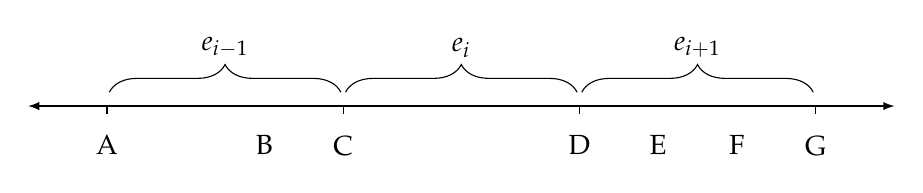
\begin{tikzpicture}
% axis
\draw[latex-latex] (0,0) -- (11,0) ;

% epoch braces
\draw [decorate,decoration={brace,amplitude=10pt} ,yshift=5pt] (1.03,0) -- (3.97,0)
  node [midway, above, yshift=9pt]{$e_{i-1}$};
\draw [decorate,decoration={brace,amplitude=10pt} ,yshift=5pt] (4.03,0) -- (6.97,0)
  node [midway, above, yshift=9pt]{$e_{i}$};
\draw [decorate,decoration={brace,amplitude=10pt} ,yshift=5pt] (7.03,0) -- (9.97,0)
  node [midway, above, yshift=9pt]{$e_{i+1}$};

% epoch boundaries
\foreach \x in  {1,4,7,10}
  \draw[shift={(\x,0)}] (0pt,0pt) -- (0pt,-3pt);

\node at (1,-0.5) {A};
\node at (3,-0.5) {B};
\node at (4,-0.5) {C};
\node at (7,-0.5) {D};
\node at (8,-0.5) {E};
\node at (9,-0.5) {F};
\node at (10,-0.5) {G};

\end{tikzpicture}

We must therefore store the last three stake distributions.
The mnemonic ``mark, set, go'' will be used to keep
track of the snapshots, where the label ``mark'' refers to the most recent snapshot,
and ``go'' refers to the snapshot that is ready to be used in the reward calculation.
In the above diagram, the snapshot taken at (A) is labeled ``mark'' during epoch $e_{i-1}$,
``set'' during epoch $e_i$ and ``go'' during epoch $e_{i+1}$. At (G) the snapshot
taken at (A) is no longer needed and will be discarded.

The two main transition systems in this section are:
\begin{itemize}
  \item The transition system named $\mathsf{EPOCH}$, which is defined in
    Section~\ref{sec:total-epoch}, covers what happens at the epoch boundary,
    such as at (A), (C), (D) and (G).
  \item The transition named $\mathsf{RUPD}$, which is defined in
    Section~\ref{sec:reward-update-trans}, covers the reward calculation that
    happens between (E) and (F).
\end{itemize}


\begin{note}
  Between time D and E we are concerned with chain growth and stability.
  Therefore this duration can be stated as 2k blocks (to state it in slots requires details about
  the particular version of the Shardagnostic protocol). The duration between F and G is also 2k blocks.
  Between E and F a single honest block is enough to ensure a random nonce.
\end{note}

\subsection{Example Illustration of the Reward Cycle}
\label{sec:illustration-reward-cycle}

\definecolor{epochColor}{rgb} {1.00,0.50,0.00}
\definecolor{aliceColor}{rgb} {0.65,0.00,0.00}
\definecolor{bobColor}{rgb} {0.00,0.50,0.00}
\definecolor{bob2Color}{rgb} {0.00,0.95,0.00}
\definecolor{snapshot1}{rgb} {0.00,0.00,0.90}
\definecolor{snapshot2}{rgb} {0.00,0.60,0.90}

\begin{tikzpicture}

  % Axis
  \draw [thick] (-0.2,0) -- (13,0);
  \draw (0,-.2) -- (0, .2);
  \draw (3,-.2) -- (3, .2);
  \draw (6,-.2) -- (6, .2);
  \draw (9,-.2) -- (9, .2);
  \draw (12,-.2) -- (12, .2);
  \node[align=center, below, color=epochColor] at (1.5,0.5)
    {$e_1$};
  \node[align=center, below, color=epochColor] at (4.5,0.5)
    {$e_2$};
  \node[align=center, below, color=epochColor] at (7.5,0.5)
    {$e_3$};
  \node[align=center, below, color=epochColor] at (10.5,0.5)
    {$e_4$};

  % Alice
  % Alice's circle
  \draw [aliceColor, fill] (0,3) circle [radius=0.5];
  \node [white] at (0,3) {Alice};
  % Alice's delegation line
  \draw [->,thick, aliceColor] (0.4,2.65) to (2,0.05);
  \node [aliceColor] at (2.2,2) {delegate to Bob};

  % Bob
  % Bob's circle
  \draw [bobColor, fill] (0,-3) circle [radius=0.5];
  \node [white] at (0,-3) {Bob};
  % Bob's registration line
  \draw [->,thick, bobColor] (0.2,-2.50) to (1,-0.05);
  \node [align=left, below, bobColor] at (-0.5,-0.5) {initial pool \\ registration};
  % Bob's re-registration line
  \draw [->,thick, bob2Color] (0.45,-2.65) to (2.90,-0.05);
  \node [bob2Color] at (2,-2.8) {re-registration};
  % Bob's cached parameter change
  \draw [->,thick, bob2Color] (2.9,-0.2) to [out=280, in=180] (3,-2)
     to [out=0, in=290] (3.1,-0.2);

  % Alice time to re-delegate
  \draw [decorate, decoration = {brace, mirror, amplitude=10pt}, aliceColor, thick]
    (3.2,-0.2) to (5.9,-0.2);
  \node [align=center, below, aliceColor] at (5.1,-0.5)
    {Alice's opportunity \\ to re-delegate \\ before Bob's new \\ parameters};

  % Bob's blocks
  % epoch e3
  \draw [fill=bobColor,bobColor] (6.3,-.1) rectangle (6.5,-.3);
  \draw [fill=bobColor,bobColor] (6.7,-.1) rectangle (6.9,-.3);
  \draw [fill=bobColor,bobColor] (7.4,-.1) rectangle (7.6,-.3);
  \draw [fill=bobColor,bobColor] (8.4,-.1) rectangle (8.6,-.3);
  \draw [decorate, decoration = {brace, mirror, amplitude=10pt}, bobColor, thick]
    (6.2, -0.4) to (8.9,-0.4);
  \draw [->,thick, bobColor] (7.6, -0.8) to [out=315,in=200] (8.4, -1.2)
     to [] (9.6, -0.9);

  % epoch e4
  \draw [fill=bob2Color,bob2Color] (9.9,-.1) rectangle (10.1,-.3);
  \draw [fill=bob2Color,bob2Color] (10.4,-.1) rectangle (10.6,-.3);
  \draw [fill=bob2Color,bob2Color] (10.8,-.1) rectangle (11.0,-.3);
  \draw [decorate, decoration = {brace, mirror, amplitude=10pt}, bob2Color, thick]
    (9.7, -0.4) to (11.2,-0.4);
  \draw [->,thick, bob2Color] (10.6, -0.8) to [out=315,in=200] (11.4, -1.2)
     to [] (12.6, -0.9);

  % Snapshots
  \draw [->,thick, snapshot1] (3,0.3) to [out=90,in=150] (9,0.5)
     to [out=330,in=180] (10,-1) to [out=0,in=-135] (12,0) ;
   \node [snapshot1] at (2.7,1.2) {mark};
   \node [snapshot1] at (6,1.9) {set};
   \node [snapshot1] at (9,0.9) {go};

  \draw [->,thick, snapshot2] (6,0.3) to [out=90,in=150] (12,0.5)
     to [out=330,in=180] (13,-1);
   \node [snapshot2] at (5.7,1.2) {mark};
   \node [snapshot2] at (9,1.9) {set};
   \node [snapshot2] at (12,0.9) {go};
\end{tikzpicture}

Bob registers his stake pool in epoch $e_1$.
Alice delegates to Bob's stake pool in epoch $e_1$.
Just before the end of epoch $e_1$, Bob submits a stake pool re-registration,
changing his pool parameters. The change in parameters is not immediate,
as shown by the curved arrow around the epoch boundary.

A snapshot is taken on the $e_1$/$e_2$ boundary. It is labeled ``mark'' initially.
This snapshot includes Alice's delegation to Bob's pool, and Bob's pool parameters
and listed in the initial pool registration certificate.

If Alice changes her delegation choice any time during epoch $e_2$,
she will never be effected by Bob's change of parameters.

A new snapshot is taken on the $e_2$/$e_3$ boundary.
The previous (darker blue) snapshot is now labeled ``set'', and the new one labeled ``mark''.
The ``set'' snapshot is used for leader election in epoch $e_3$.

On the $e_3$/$e_4$ boundary, the darker blue snapshot is labeled ``go'' and
the lighter blue snapshot is labeled ``set''.
Bob's stake pool performance during epoch $e_3$ (he produced 4 blocks)
will be used with the darker blue snapshot for the rewards which will
be handed out at the beginning of epoch $e_5$.

\subsection{Helper Functions and Accounting Fields}
\label{sec:stake-dist-helpers}

Figure~\ref{fig:funcs:epoch-helper-rewards} defines four helper functions needed
throughout the rest of the section.

\begin{itemize}
  \item The function $\fun{obligation}$ calculates the the minimal amount of coin needed to
    pay out all deposit refunds.
  \item The function $\fun{poolStake}$ filters the stake distribution to one stake pool.
\end{itemize}


%%
%% Figure - Helper Functions for Epoch Rules
%%
\begin{figure}[htb]
  \emph{Total possible refunds}
  \begin{align*}
    & \fun{obligation} \in \PParams \to (\StakeCredential \mapsto \Coin)
    \to (\KeyHash_{pool}\mapsto\PoolParam) \to \Coin \\
    & \obligation{pp}{rewards}{poolParams} = \\
    & ~~~~~
    (\fun{keyDeposit}~\var{pp}) \cdot|\var{rewards}| +
    (\fun{poolDeposit}~\var{pp}) \cdot|\var{poolParams}| \\
  \end{align*}
  %
  \emph{Filter Stake to one Pool}
  \begin{align*}
      & \fun{poolStake} \in \KeyHash_{pool} \to (\KeyHash_{stake} \mapsto \KeyHash_{pool})
        \to \Stake \to \Stake \\
      & \poolStake{hk}{delegs}{stake} =
        \dom{(\var{delegs}\restrictrange\{hk\})\restrictdom\var{stake}}
  \end{align*}

  \caption{Helper Functions used in Rewards and Epoch Boundary}
  \label{fig:funcs:epoch-helper-rewards}
\end{figure}


The Figure~\ref{fig:defs:accounting} lists the accounting fields, denoted by $\Acnt$,
which will be used throughout this section. It consists of:
\begin{itemize}
  \item The value $\var{treasury}$ tracks the amount of coin currently stored in the treasury.
    Initially there will be no way to remove these funds.
  \item The value $\var{reserves}$ tracks the amount of coin currently stored in the reserves.
    This pot is used to pay rewards.
\end{itemize}
More will be said about the general accounting system in Section~\ref{sec:reward-calc}.

%%
%% Figure - Accounting fields
%%
\begin{figure}[htb]
  \emph{Accounting Fields}
  \begin{equation*}
    \Acnt =
    \left(
      \begin{array}{r@{~\in~}ll}
        \var{treasury} & \Coin & \text{treasury pot}\\
        \var{reserves} & \Coin & \text{reserve pot}\\
      \end{array}
    \right)
  \end{equation*}
  %
  \caption{Accounting fields}
  \label{fig:defs:accounting}
\end{figure}


\subsection{Stake Distribution Calculation}
\label{sec:stake-dist-calc}

This section defines the stake distribution calculations.
Figure~\ref{fig:epoch-defs} introduces three new derived types:
\begin{itemize}
  \item $\type{BlocksMade}$ represents the number of blocks each stake pool produced
    during an epoch.
  \item $\type{Stake}$ represents the amount of stake (in $\type{Coin}$) controlled by each
    stake pool.
\end{itemize}

%%
%% Figure - Epoch Abstract Types
%%
\begin{figure}[htb]
  \emph{Derived types}
  %
  \begin{equation*}
    \begin{array}{r@{~\in~}l@{\qquad=\qquad}lr}
      \var{blocks}
      & \BlocksMade
      & \KeyHash_{pool} \mapsto \N
      & \text{blocks made by stake pools} \\
      \var{stake}
      & \Stake
      & \Credential \mapsto \Coin
      & \text{stake} \\
    \end{array}
  \end{equation*}
  \caption{Epoch definitions}
  \label{fig:epoch-defs}
\end{figure}

The stake distribution calculation is given in Figure~\ref{fig:functions:stake-distribution}.

\begin{itemize}
\item $\fun{aggregate_{+}}$ takes a relation on $A\times B$, where $B$ is any
  monoid $(B,+,e)$ and returns a map from each $a\in A$ to the ``sum'' (using
  the monoidal $+$ operation) of all $b\in B$ such that $(a, b)\in A\times B$.
\item $\fun{stakeDistr}$ uses the $\fun{aggregate_{+}}$ function and several relations to
    compute the stake distribution, mapping each hashkey to the total coin under its control.
    Keys that are not both registered and delegated are filtered out.
    The relation passed to $\fun{aggregate_{+}}$ is made up of:
    \begin{itemize}
      \item $\fun{stakeCred_b}^{-1}$, relating credentials to (base) addresses
      \item $\left(\fun{addrPtr}\circ\var{ptr}\right)^{-1}$, relating credentials to (pointer)
        addresses
      \item $\range{utxo}$, relating addresses to coins
      \item $\fun{stakeCred_r}^{-1}\circ\var{rewards}$, relating (reward) addresses to coins
    \end{itemize}
    The notation for relations is explained in Section~\ref{sec:notation-sophie}.
\end{itemize}

%%
%% Figure Functions for Stake Distribution
%%
\begin{figure}[htb]
  \emph{Aggregation (for a monoid B)}
  %
  \begin{align*}
      & \fun{aggregate_{+}} \in \powerset{(A \times B)} \to (A\mapsto B) \\
      & \fun{aggregate_{+}}~\var{R} = \left\{a\mapsto \sum_{(a,b)\in\var{R}}b
          ~\mid~a\in\dom\var{R}\right\} \\
  \end{align*}
  %
  \emph{Stake Distribution (using functions and maps as relations)}
  %
  \begin{align*}
      & \fun{stakeDistr} \in \UTxO \to \DState \to \PState \to \Snapshot \\
      & \fun{stakeDistr}~{utxo}~{dstate}~{pstate} = \\
      & ~~~~ \big((\dom{\var{activeDelegs}})
      \restrictdom\left(\fun{aggregate_{+}}~\var{stakeRelation}\right),
    ~\var{delegations},~\var{poolParams}\big)\\
      & \where \\
      & ~~~~ (~\var{rewards},~\var{delegations},~\var{ptrs},~\wcard,~\wcard,~\wcard)
        = \var{dstate} \\
      & ~~~~ (~\var{poolParams},~\wcard,~\wcard) = \var{pstate} \\
      & ~~~~ \var{stakeRelation} = \left(
        \left(\fun{stakeCred_b}^{-1}\cup\left(\fun{addrPtr}\circ\var{ptr}\right)^{-1}\right)
        \circ\left(\range{\var{utxo}}\right)
        \right)
        \cup \var{rewards} \\
      & ~~~~ \var{activeDelegs} =
               (\dom{rewards}) \restrictdom \var{delegations} \restrictrange (\dom{poolParams}) \\
  \end{align*}

  \caption{Stake Distribution Function}
  \label{fig:functions:stake-distribution}
\end{figure}

\clearpage

\subsection{Snapshot Transition}
\label{sec:snapshots}

The state transition types for stake distribution snapshots are given in
Figure~\ref{fig:ts-types:snapshot}.
Each snapshot consists of:
\begin{itemize}
  \item $\var{stake}$, a stake distribution, which is defined in
    Figure~\ref{fig:epoch-defs} as a mapping of credentials to coin.
  \item $\var{delegations}$, a delegation map, mapping credentials to stake pools.
  \item $\var{poolParameters}$, storing the pool parameters of each stake pool.
\end{itemize}

The type $\type{\Snapshots}$ contains the
information needing to be saved on the epoch boundary:
\begin{itemize}
  \item $\var{pstake_{mark}}$, $\var{pstake_{set}}$ and $\var{pstake_{go}}$ are the three
    snapshots as explained in Section~\ref{sec:reward-overview}.
  \item $\var{feeSS}$ stores the fees which are added to the reward pot during
    the next reward update calculation, which is then subtracted from the fee pot
    on the epoch boundary.
\end{itemize}

%%
%% Figure - Snapshots Defs
%%
\begin{figure}[htb]
  \emph{Snapshots}
  \begin{equation*}
    \Snapshot =
    \left(
      \begin{array}{r@{~\in~}ll}
        \var{stake} & \Stake & \text{stake distribution}\\
        \var{delegations} & \Credential\mapsto\KeyHash_{pool}
                          & \text{stake delegations}\\
        \var{poolParameters} & \KeyHash_{pool} \mapsto \PoolParam & \text{pool parameters }\\
      \end{array}
    \right)
  \end{equation*}

  \begin{equation*}
    \Snapshots =
    \left(
      \begin{array}{r@{~\in~}ll}
        \var{pstake_{mark}} & \Snapshot & \text{newest stake}\\
        \var{pstake_{set}}  & \Snapshot & \text{middle stake}\\
        \var{pstake_{go}}   & \Snapshot & \text{oldest stake}\\
        \var{feeSS} & \Coin & \text{fee snapshot}\\
      \end{array}
    \right)
  \end{equation*}
  %
  \emph{Snapshot transitions}
  \begin{equation*}
    \_ \vdash
    \var{\_} \trans{snap}{} \var{\_}
    \subseteq \powerset (\LState \times \Snapshots \times \Snapshots)
  \end{equation*}
  %
  \caption{Snapshot transition-system types}
  \label{fig:ts-types:snapshot}
\end{figure}

The snapshot transition rule is given in Figure~\ref{fig:rules:snapshot}.
This transition has no preconditions and results in the following state change:

\begin{itemize}
  \item The oldest snapshot is replaced with the penultimate one.
  \item The penultimate snapshot is replaced with the newest one.
  \item The newest snapshot is replaced with one just calculated.
  \item The current fees pot is stored in $\var{feeSS}$. Note that this value will not
    change during the epoch, unlike the $\var{fees}$ value in the UTxO state.
\end{itemize}

%%
%% Figure - Snapshot Rule
%%
\begin{figure}[htb]
  \begin{equation}\label{eq:snapshot}
    \inference[Snapshot]
    {
      {
      \begin{array}{r@{~\leteq~}l}
        ((\var{utxo},~\wcard,\var{fees},~\wcard),~(\var{dstate},~\var{pstate})) & \var{lstate} \\
        \var{stake} & \stakeDistr{utxo}{dstate}{pstate} \\
      \end{array}
      }
    }
    {
      \begin{array}{r}
        \var{lstate} \\
      \end{array}
      \vdash
      \left(
        \begin{array}{r}
          \var{pstake_{mark}}\\
          \var{pstake_{set}}\\
          \var{pstake_{go}}\\
          \var{feeSS} \\
        \end{array}
      \right)
      \trans{snap}{}
      \left(
        \begin{array}{r}
          \varUpdate{\var{stake}} \\
          \varUpdate{\var{pstake_{mark}}} \\
          \varUpdate{\var{pstake_{set}}} \\
          \varUpdate{\var{fees}} \\
        \end{array}
      \right)
    }
  \end{equation}
  \caption{Snapshot Inference Rule}
  \label{fig:rules:snapshot}
\end{figure}

\clearpage

\subsection{Pool Reaping Transition}
\label{sec:pool-reap}

Figure~\ref{fig:ts-types:pool-reap} defines the types for the pool reap transition,
which is responsible for removing pools slated for retirement in the given epoch.

%%
%% Figure - Pool Reap Defs
%%
\begin{figure}[htb]
  \emph{Pool Reap State}
  \begin{equation*}
    \PlReapState =
    \left(
      \begin{array}{r@{~\in~}ll}
        \var{utxoSt} & \UTxOState & \text{utxo state}\\
        \var{acnt} & \Acnt & \text{accounting}\\
        \var{dstate} & \DState & \text{delegation state}\\
        \var{pstate} & \PState & \text{pool state}\\
      \end{array}
    \right)
  \end{equation*}
  %
  \emph{Pool Reap transitions}
  \begin{equation*}
    \_ \vdash \_ \trans{poolreap}{\_} \_ \in
    \powerset (\PParams \times \PlReapState \times \Epoch \times \PlReapState)
  \end{equation*}
  %
  \caption{Pool Reap Transition}
  \label{fig:ts-types:pool-reap}
\end{figure}


The pool-reap transition rule is given in Figure~\ref{fig:rules:pool-reap}.
This transition has no preconditions and results in the following state change:

\begin{itemize}
  \item For each retiring pool, the refund for the pool registration deposit is added to the
    pool's registered reward account, provided the reward account is still registered.
  \item The sum of all the refunds attached to unregistered reward accounts are added to the
    treasury.
  \item The deposit pool is reduced by the amount of claimed and unclaimed refunds.
  \item Any delegation to a retiring pool is removed.
  \item Each retiring pool is removed from all four maps in the pool state.
\end{itemize}

%%
%% Figure - Pool Reap Rule
%%
\begin{figure}[htb]
  \begin{equation}\label{eq:pool-reap}
    \inference[Pool-Reap]
    {
      {
      \begin{array}{r@{~\leteq~}l}
        \var{retired} & \dom{(\var{retiring}^{-1}~\var{e})} \\
        \var{pr} & \left\{
                   \var{hk}\mapsto(\fun{poolDeposit}~\var{pp})
                     \mid
                     \var{hk}\in\var{retired}
                   \right\}\\
        \var{rewardAcnts}
                 & \{\var{hk}\mapsto \fun{poolRAcnt}~\var{pool} \mid
                   \var{hk}\mapsto\var{pool} \in \var{retired}\restrictdom\var{poolParams} \} \\
        \var{rewardAcnts'} & \left\{
                        a \mapsto c
                        \mathrel{\Bigg|}
                        \begin{array}{r@{~\in~}l}
                          \var{hk} \mapsto c & \var{pr}, \\
                          \var{hk}\mapsto\var{a} & \var{rewardAcnts} \\
                        \end{array}
                      \right\} \\
        \var{refunds} & \dom{rewards}\restrictdom\var{rewardAcnts'} \\
        \var{mRefunds} & \dom{rewards}\subtractdom\var{rewardAcnts'} \\
        \var{refunded} & \sum\limits_{\wcard\mapsto c\in\var{refunds}} c \\
        \var{unclaimed} & \sum\limits_{\wcard\mapsto c\in\var{mRefunds}} c \\
      \end{array}
      }
    }
    {
      \var{pp}
      \vdash
      \left(
        \begin{array}{r}
          \var{utxo} \\
          \var{deposited} \\
          \var{fees} \\
          \var{ppup} \\
          ~ \\
          \var{treasury} \\
          \var{reserves} \\
          ~ \\
          \var{rewards} \\
          \var{delegations} \\
          \var{ptrs} \\
          \var{genDelegs} \\
          \var{fGenDelegs} \\
          \var{i_{rwd}} \\
          ~ \\
          \var{poolParams} \\
          \var{fPoolParams} \\
          \var{retiring} \\
        \end{array}
      \right)
      \trans{poolreap}{e}
      \left(
        \begin{array}{rcl}
          \var{utxo} \\
          \varUpdate{\var{deposited}}
          & \varUpdate{-}
          & \varUpdate{(\var{unclaimed} + \var{refunded})} \\
          \var{fees} \\
          \var{ppup} \\
          ~ \\
          \varUpdate{\var{treasury}} & \varUpdate{+} & \varUpdate{\var{unclaimed}} \\
          \var{reserves} \\
          ~ \\
          \varUpdate{\var{rewards}} & \varUpdate{\unionoverridePlus} & \varUpdate{\var{refunds}} \\
          \varUpdate{\var{delegations}} & \varUpdate{\subtractrange} & \varUpdate{\var{retired}} \\
          \var{ptrs} \\
          \var{genDelegs} \\
          \var{fGenDelegs} \\
          \var{i_{rwd}}\\
          ~ \\
          \varUpdate{\var{retired}} & \varUpdate{\subtractdom} & \varUpdate{\var{poolParams}} \\
          \varUpdate{\var{retired}} & \varUpdate{\subtractdom} & \varUpdate{\var{fPoolParams}} \\
          \varUpdate{\var{retired}} & \varUpdate{\subtractdom} & \varUpdate{\var{retiring}} \\
        \end{array}
      \right)
    }
  \end{equation}
  \caption{Pool Reap Inference Rule}
  \label{fig:rules:pool-reap}
\end{figure}

\clearpage

\subsection{Protocol Parameters Update Transition}
\label{sec:pparam-update}

Finally, reaching the epoch boundary may trigger a change in the protocol parameters.
The protocol parameters environment consists of the delegation and pool states,
and the signal is an optional new collection of protocol parameters
The state change is a change of the $\UTxOState$, the $\Acnt$ states and the current $\PParams$.
The type of this state transition is given in Figure~\ref{fig:ts-types:new-proto-param}.

%%
%% Figure - New Proto Param Defs
%%
\begin{figure}[htb]
  \emph{New Proto Param environment}
  \begin{equation*}
    \NewPParamEnv =
    \left(
      \begin{array}{r@{~\in~}ll}
        \var{dstate} & \DState & \text{delegation state}\\
        \var{pstate} & \PState & \text{pool state}\\
      \end{array}
    \right)
  \end{equation*}
  %
  \emph{New Proto Param States}
  \begin{equation*}
    \NewPParamState =
    \left(
      \begin{array}{r@{~\in~}ll}
        \var{utxoSt} & \UTxOState & \text{utxo state}\\
        \var{acnt} & \Acnt & \text{accounting}\\
        \var{pp} & \PParams & \text{current protocol parameters}\\
      \end{array}
    \right)
  \end{equation*}
  %
  \emph{New Proto Param transitions}
  \begin{equation*}
    \_ \vdash
    \var{\_} \trans{newpp}{\_} \var{\_}
    \subseteq \powerset (\NewPParamEnv \times \NewPParamState \times \PParams^? \times \NewPParamState)
  \end{equation*}
  %
  \caption{New Proto Param transition-system types}
  \label{fig:ts-types:new-proto-param}
  %
  \emph{Helper Functions}
  \begin{align*}
      & \fun{updatePpup} \in \UTxOState \to \PParams \to \UTxOState\\
      & \fun{updatePpup}~\var{utxoSt}~\var{pp} =
      \begin{cases}
        (\var{utxo},\var{deposited},\var{fees},(\var{fpup},~\emptyset))
        &
        \var{canFollow}
        \\
        (\var{utxo},\var{deposited},\var{fees},(\emptyset,~\emptyset))
        &
        \text{otherwise} \\
      \end{cases}\\
      & ~~~\where \\
      & ~~~~~~~\var{canFollow} =
        \forall\var{ps}\in\range{pup},~
        \var{pv}\mapsto\var{v}\in\var{ps}\implies\fun{pvCanFollow}~(\fun{pv}~\var{pp})~\var{v}
        \\
      & ~~~~~~~(\var{utxo},\var{deposited},\var{fees},(\var{pup},~\var{fpup})) = \var{utxoSt} \\
  \end{align*}
\end{figure}


Figure~\ref{fig:rules:new-proto-param} defines the new protocol parameter transition.
The transition has two rules, depending on whether or not the new protocol parameters
meet some requirements.
In particular, we require that the new parameters would not incur a debt of the system that
can not be covered by the reserves, and that the max block size is greater than the sum of the
max transaction size and the max header size.
If the requirements are met, the new protocol parameters are accepted, the proposal is reset,
and the reserves are adjusted to account for changes in the deposits.
Otherwise, the only change is that the proposal is reset.

The $\mathsf{NEWPP}$ rule also cleans up the protocol parameter update proposals,
by calling $\fun{updatePpup}$ on the UTxO state.
The $\fun{updatePpup}$ sets the protocol parameter updates to the future protocol
parameter updates provided the protocol versions all can follow from the
version given in the protocol parameters, or the emptyset otherwise.
In any case, the future protocol parameters update proposals are set to the empty set.
If new protocol parameters are being adopted, then these is the value given to
$\fun{updatePpup}$, otherwise the old parameters are given.

Regarding adjusting the reserves for changes in the deposits, one of three things happens:

\begin{itemize}
  \item If the new protocol parameters mean that \textbf{fewer} funds are required in the
    deposit pot to cover all possible refunds, then the excess is moved to the reserves.

  \item If the new protocol parameters mean that \textbf{more} funds are required in the
    deposit pot to cover all possible refunds and the difference is \textbf{less} than
    the reserve pot, then funds are moved from the reserve pot to cover the difference.

  \item If the new protocol parameters mean that \textbf{more} funds are required in the
    deposit pot to cover all possible refunds and the difference is \textbf{more} than
    the reserve pot, then Rule~\ref{eq:new-pc-denied} meets the precondition and the
    only change of state is that the update proposals are reset.
\end{itemize}

Note that here, unlike most of the inference rules in this document,
the $\var{utxoSt'}$ and the $\var{acnt'}$ do not come from valid UTxO or
accounts transitions in the antecedent. We simply define the consequent
transition using these directly (instead of listing all the fields in both
states in the consequent transition). It is done this way here
for ease of reading.

%%
%% Figure - New Proto Param Rule
%%
\begin{figure}[htb]
  \begin{equation}\label{eq:new-pc-accepted}
    \hspace{-0.3cm}
    \inference[New-Proto-Param-Accept]
    {
      \var{pp_{new}}\neq\Nothing \\~\\
      {\begin{array}{rcl}
         (\var{utxo},~\var{deposited},~\var{fees},~\var{ppup}) & \leteq & \var{utxoSt} \\
         \var{(\var{rewards},~\wcard,~\wcard,~\wcard,~\wcard,~\var{i_{rwd}})} &
         \leteq & \var{dstate}\\
         \var{(\var{poolParams},~\wcard,~\wcard)} & \leteq & \var{pstate}\\
         \var{oblg_{cur}} & \leteq & \obligation{pp}{rewards}{poolParams} \\
         \var{oblg_{new}} & \leteq & \obligation{pp_{new}}{rewards}{poolParams} \\
         \var{diff} & \leteq & \var{oblg_{cur}} - \var{oblg_{new}}\\
      \end{array}}
      \\~\\~\\
      \var{oblg_{cur}} = \var{deposited} \\
      \var{reserves} + \var{diff} \geq \sum\limits_{\wcard\mapsto\var{val}\in\var{i_{rwd}}} val \\
      \fun{maxTxSize}~\var{pp_{new}} + \fun{maxHeaderSize}~\var{pp_{new}} <
        \fun{maxBlockSize}~\var{pp_{new}}
      \\~\\
        \var{utxoSt'} \leteq
        \left(\var{utxo},~\varUpdate{oblg_{new}},~\var{fees},~\var{ppup}\right)
      \\
      \var{utxoSt''} \leteq \fun{updatePpup}~\var{utxoSt'}~\var{pp_{new}}
      \\~\\
      (\var{treasury},~\var{reserves})\leteq \var{acnt} \\
      \var{acnt'} \leteq (\var{treasury},~\varUpdate{reserves + diff}) \\
    }
    {
      \begin{array}{l}
        \var{dstate}\\
        \var{pstate}\\
      \end{array}
      \vdash
      \left(
        \begin{array}{r}
          \var{utxoSt} \\
          \var{acnt} \\
          \var{pp}
        \end{array}
      \right)
      \trans{newpp}{\var{pp_{new}}}
      \left(
        \begin{array}{rcl}
          \varUpdate{utxoSt''}\\
          \varUpdate{acnt'} \\
          \varUpdate{\var{pp_{new}}} \\
        \end{array}
      \right)
    }
  \end{equation}

  \nextdef

  \begin{equation}\label{eq:new-pc-denied}
    \inference[New-Proto-Param-Denied]
    {
      \left({\begin{array}{c}
            \var{pp_{new}}=\Nothing \\
        \lor \\
        \var{reserves} + \var{diff} < \sum\limits_{\wcard\mapsto\var{val}\in\var{i_{rwd}}} val\\
        \lor \\
        \fun{maxTxSize}~\var{pp_{new}} + \fun{maxHeaderSize}~\var{pp_{new}} \geq
          \fun{maxBlockSize}~\var{pp_{new}}
      \end{array}}\right)
      \\~\\~\\
      {\begin{array}{rcl}
          \var{(\var{rewards},~\wcard,~\wcard,~\wcard,~\wcard,~\var{i_{rwd}})} &
          \leteq & \var{dstate}\\
         \var{(\var{poolParams},~\wcard,~\wcard)} & \leteq & \var{pstate}\\
          \var{oblg_{cur}} & \leteq & \obligation{pp}{rewards}{poolParams} \\
          \var{oblg_{new}} & \leteq & \obligation{pp_{new}}{rewards}{poolParams} \\
         \var{diff} & \leteq & \var{oblg_{cur}} - \var{oblg_{new}}
      \end{array}}
      \\~\\~\\
      \var{utxoSt'} \leteq \fun{updatePpup}~\var{utxoSt}~\var{pp} \\
    }
    {
      \begin{array}{l}
        \var{dstate}\\
        \var{pstate}\\
      \end{array}
      \vdash
      \left(
        \begin{array}{r}
          \var{utxoSt} \\
          \var{acnt} \\
          \var{pp}
        \end{array}
      \right)
      \trans{newpp}{\var{pp_{new}}}
      \left(
        \begin{array}{rcl}
          \varUpdate{utxoSt'}\\
          \var{acnt} \\
          \var{pp}
        \end{array}
      \right)
    }
  \end{equation}
  \caption{New Proto Param Inference Rule}
  \label{fig:rules:new-proto-param}
\end{figure}

\clearpage

\subsection{Complete Epoch Boundary Transition}
\label{sec:total-epoch}

Finally, it is possible to define the complete epoch boundary transition type,
which is defined in Figure~\ref{fig:ts-types:epoch}.
The transition has no evironment.
The state is made up of the the accounting state, the snapshots, the ledger state and the
protocol parameters.
The transition uses a helper function $\fun{votedValue}$ which returns
the consensus value of update proposals in the event that consensus is met.
\textbf{Note that} $\fun{votedValue}$
\textbf{is only well-defined if } $\var{quorum}$
\textbf{is greater than half the number of core nodes, i.e.}
$\Quorum > |\var{genDelegs}|/2$ \textbf{.}

%%
%% Figure - Epoch Defs
%%
\begin{figure}[htb]
  \emph{Epoch States}
  \begin{equation*}
    \EpochState =
    \left(
      \begin{array}{r@{~\in~}ll}
        \var{acnt} & \Acnt & \text{accounting}\\
        \var{ss} & \Snapshots & \text{snapshots}\\
        \var{ls} & \LState & \text{ledger state}\\
        \var{prevPp} & \PParams & \text{previous protocol parameters}\\
        \var{pp} & \PParams & \text{protocol parameters}\\
      \end{array}
    \right)
  \end{equation*}
  %
  \emph{Epoch transitions}
  \begin{equation*}
    \vdash
    \var{\_} \trans{epoch}{\_} \var{\_}
    \subseteq \powerset (\EpochState \times \Epoch \times \EpochState)
  \end{equation*}
  %
  \emph{Accessor Functions}
  \begin{equation*}
    \begin{array}{r@{~\in~}lr}
      \fun{getIR} & \EpochState \to (\StakeCredential \mapsto \Coin)
                  & \text{get instantaneous rewards} \\
    \end{array}
  \end{equation*}
  %
  \emph{Helper Functions}
  \begin{align*}
      & \fun{votedValue} \in (\KeyHashGen\mapsto\PParamsUpdate) \to \PParams \to \N \to \PParamsUpdate^?\\
      & \fun{votedValue}~\var{pup}~\var{pp}~\var{quorum} =
      \begin{cases}
        \var{pp}\unionoverrideRight\var{p}
          & \exists! p\in\range{pup}~(|pup\restrictrange p|\geq \var{quorum}) \\
        \Nothing & \text{otherwise} \\
      \end{cases}
  \end{align*}
  %
  \caption{Epoch transition-system types}
  \label{fig:ts-types:epoch}
\end{figure}


The epoch transition rule calls $\mathsf{SNAP}$, $\mathsf{POOLREAP}$ and $\mathsf{NEWPP}$
in sequence. It also stores the previous protocol parameters in $\var{prevPp}$.
The previous protocol parameters will be used for the reward calculation in the upcoming epoch,
note that they correspond to the epoch for which the rewards are being calculated.
Additionally, this transition also adopts the pool parameters $\var{fPoolParams}$
corresponding to the pool re-registration certificates which we submitted late in the ending epoch.
The ordering of these rules is important.
The stake pools which will be updated by $\var{fPoolParams}$ or
reaped during the $\mathsf{POOLREAP}$ transition must still be a
part of the new snapshot, and so $\mathsf{SNAP}$ must occur before these two actions.
Moreover, $\mathsf{SNAP}$ sets the deposit pot equal to current obligation,
which is a property that is preserved by $\mathsf{POOLREAP}$ and which
is necessary for the preservation of Bcc property in the $ \mathsf{NEWPP}$ transition.

%%
%% Figure - Epoch Rule
%%
\begin{figure}[htb]
  \begin{equation}\label{eq:epoch}
    \inference[Epoch]
    {
      {
        \begin{array}{r}
          \var{lstate} \\
        \end{array}
      }
      \vdash
      { \var{ss} }
      \trans{\hyperref[fig:rules:snapshot]{snap}}{}
      { \var{ss'} }
      \\~\\
      (\var{utxoSt},~(\var{dstate},~\var{pstate}))\leteq\var{ls} \\
      (\var{poolParams},~\var{fPoolParams},~\var{retiring})\leteq\var{pstate}
      \\
      \var{pstate'}\leteq(\var{poolParams}\unionoverrideRight\var{fPoolParams},
      ~\emptyset,~\var{retiring})
      \\~\\~\\
      \var{pp}
      \vdash
      \left(
        {
          \begin{array}{r}
            \var{utxoSt} \\
            \var{acnt} \\
            \var{dstate} \\
            \var{pstate'} \\
          \end{array}
        }
      \right)
      \trans{\hyperref[fig:rules:pool-reap]{poolreap}}{e}
      \left(
      {
        \begin{array}{rcl}
            \var{utxoSt'} \\
            \var{acnt'} \\
            \var{dstate'} \\
            \var{pstate''} \\
        \end{array}
      }
      \right)
      \\~\\~\\
      \var{(\wcard,~\wcard,~\wcard,~(\var{pup},\wcard))}\leteq\var{utxoSt'}\\
      \var{pp_{new}}\leteq\fun{votedValue}~\var{pup}~\var{pp}~\Quorum\\
      {
        \begin{array}{r}
          \var{dstate'}\\
          \var{pstate''}\\
        \end{array}
      }
      \vdash
      \left(
        {
          \begin{array}{r}
            \var{utxoSt'} \\
            \var{acnt'} \\
            \var{pp}\\
          \end{array}
        }
      \right)
      \trans{\hyperref[fig:rules:new-proto-param]{newpp}}{\var{pp_{new}}}
      \left(
      {
        \begin{array}{rcl}
            \var{utxoSt''} \\
            \var{acnt''} \\
            \var{pp'}\\
        \end{array}
      }
      \right)
      \\~\\~\\
      \var{ls}' \leteq (\var{utxoSt}'',~(\var{dstate}',~\var{pstate}''))
    }
    {
      \vdash
      \left(
      \begin{array}{r}
        \var{acnt} \\
        \var{ss} \\
        \var{ls} \\
        \var{prevPp} \\
        \var{pp} \\
      \end{array}
      \right)
      \trans{epoch}{e}
      \left(
      \begin{array}{rcl}
        \varUpdate{\var{acnt''}} \\
        \varUpdate{\var{ss'}} \\
        \varUpdate{\var{ls'}} \\
        \varUpdate{\var{pp}} \\
        \varUpdate{\var{pp'}} \\
      \end{array}
      \right)
    }
  \end{equation}
  \caption{Epoch Inference Rule}
  \label{fig:rules:epoch}
\end{figure}

\clearpage

\subsection{Rewards Distribution Calculation}
\label{sec:reward-dist}

This section defines the reward calculation for the proof of stake leader election.
Figure~\ref{fig:functions:rewards} defines the pool reward as described in section
5.5.2 of~\cite{delegation_design}.

\begin{itemize}
  \item The function $\fun{maxPool}$ gives the maximum reward a stake pool can receive in an epoch.
    This is a fraction of the total available rewards for the epoch.
    The result depends on the pool's relative stake, the pool's pledge and the following
    protocol parameters:
    \begin{itemize}
      \item $\var{a_0}$, the leader-stake influence
      \item $n_{opt}$, the optimal number of saturated stake pools
    \end{itemize}
  \item The function $\fun{mkApparentPerformance}$ computes the apparent performance of a stake pool.
    It depends on the protocol parameter $d$, the relative stake $\sigma$, the number $n$ of blocks
    the pool added to the chain and the total number $\overline{N}$ of blocks added to the chain in
    the last epoch.

\end{itemize}

%%
%% Figure - Functions for the Reward Calculation
%%
\begin{figure}[htb]
  \emph{Maximal Reward Function, called $f(s,\sigma)$ in section 5.5.2 of~\cite{delegation_design}}
  %
  \begin{align*}
      & \fun{maxPool} \in \PParams \to \Coin \to \unitInterval \to \unitInterval \to \Coin \\
      & \fun{maxPool}~\var{pp}~\var{R}~\sigma~\var{p_r} =
          ~~~\floor*{
             \frac{R}{1 + a_0}
             \cdot
             \left(
               \sigma' + p'\cdot a_0\cdot\frac{\sigma' - p'\frac{z_0-\sigma'}{z_0}}{z_0}
             \right)} \\
      & ~~~\where \\
      & ~~~~~~~a_0 = \fun{influence}~pp \\
      & ~~~~~~~n_{opt} = \fun{nopt}~pp \\
      & ~~~~~~~z_0 = 1/n_{opt} \\
      & ~~~~~~~\sigma'=\min(\sigma,~z_0) \\
      & ~~~~~~~p'=\min(p_r,~z_0) \\
  \end{align*}

  \emph{Apparent Performance, called $\hat{p}$ in section 5.5.2 of~\cite{delegation_design}}
  %
  \begin{align*}
      & \fun{mkApparentPerformance} \in \unitInterval \to \unitInterval \to \N \to \N \to \Q \\
      & \mkApparentPerformance{d}{\sigma}{n}{\overline{N}} =
        \begin{cases}
          \frac{\beta}{\sigma} & \text{if } d < 0.8 \\
          1 & \text{otherwise}
        \end{cases} \\
      & ~~~\where \\
      & ~~~~~~~\beta = \frac{n}{\max(1, \overline{N})} \\
  \end{align*}
  \caption{Functions used in the Reward Calculation}
  \label{fig:functions:rewards}
\end{figure}

\clearpage

Figure~\ref{fig:functions:reward-splitting} gives the calculation for
splitting the pool rewards with its members, as described in 6.5.2 of \cite{delegation_design}.
The portion of rewards allocated to the pool operator and owners is different
than that of the members.

\begin{itemize}
  \item The $\fun{r_{operator}}$ function calculates the leader reward, based on the pool cost,
    margin and the proportion of the pool's total stake.  Note that this reward will go to the
    reward account specified in the pool registration certificate.
  \item The $\fun{r_{member}}$ function calculates the member reward, proportionally to their
    stake after the cost and margin are removed.
\end{itemize}

%%
%% Figure - Functions for the Reward Splitting
%%
\begin{figure}[htb]
  \emph{Pool leader reward, from section 5.5.3 of \cite{delegation_design}}
  %
  \begin{align*}
      & \fun{r_{operator}} \in \Coin \to \PoolParam \to \unitInterval \to \unitIntervalNonNull \to \Coin \\
      & \lReward{\hat{f}}{pool}{s}{\sigma} =
        \begin{cases}
        \hat{f} & \hat{f} \leq c\\
        c + \floor*{(\hat{f} - c)\cdot\left(m + (1-m)\cdot\frac{s}{\sigma}\right) }&
        \text{otherwise.}
      \end{cases} \\
      & ~~~\where \\
      & ~~~~~~~c = \fun{poolCost}~pool \\
      & ~~~~~~~m = \fun{poolMargin}~pool \\
  \end{align*}

  \emph{Pool member reward, from section 5.5.3 of \cite{delegation_design}}
  %
  \begin{align*}
    & \fun{r_{member}} \in \Coin \to \PoolParam \to \unitInterval \to \unitIntervalNonNull \to \Coin \\
    & \mReward{\hat{f}}{pool}{t}{\sigma} =
      \begin{cases}
        0 & \hat{f} \leq c\\
        \floor*{(\hat{f} - c)\cdot(1-m)\cdot\frac{t}{\sigma}} &
        \text{otherwise.}
      \end{cases} \\
    & ~~~\where \\
    & ~~~~~~~c = \fun{poolCost}~pool \\
    & ~~~~~~~m = \fun{poolMargin}~pool \\
  \end{align*}

  \caption{Functions used in the Reward Splitting}
  \label{fig:functions:reward-splitting}
\end{figure}


Finally, the full reward calculation is presented in Figure~\ref{fig:functions:reward-calc}.
The calculation is done pool-by-pool.
\begin{itemize}
\item The $\fun{rewardOnePool}$ function calculates the rewards given out to
  each member of a given pool. The pool leader is identified by the stake
  credential of the pool operator. The function returns the rewards, calculated
  as follows:
    \begin{itemize}
      \item $\var{pstake}$, the total amount of stake controlled by the stake pool.
      \item $\var{ostake}$, the total amount of stake controlled by the stake pool operator
        and owners
      \item $\sigma$, the total proportion of stake controlled by the stake pool.
      \item $\overline{N}$, the expected number of blocks the pool should have produced.
      \item $\var{pledge}$, the pool's pledge in entropic.
      \item $p_r$, the pool's pledge, as a proportion of active stake.
      \item $\var{maxP}$, maximum rewards the pool can claim if the pledge is met,
        and zero otherwise.
      \item $\var{poolR}$, the pool's actual reward, based on its performance.
      \item $\var{mRewards}$, the member's rewards as a mapping of reward accounts to coin.
      \item $\var{lReward}$, the leader's reward as coin.
      \item $\var{potentialRewards}$, the combination of $\var{mRewards}$ and $\var{lRewards}$.
      \item $\var{rewards}$, the restriction of $\var{potentialRewards}$ to the active
        reward accounts.
    \end{itemize}
  \item The $\fun{reward}$ function applies $\fun{rewardOnePool}$ to each registered stake pool.
\end{itemize}

%%
%% Figure - The Reward Calculation
%%
\begin{figure}[htb]
  \emph{Calculation to reward a single stake pool}
  %
  \begin{align*}
    & \fun{rewardOnePool} \in \PParams \to \Coin \to \N \to \N \to \PoolParam\\
      & ~~~\to \Stake \to \Q \to \Q \to \Coin \to \powerset{\AddrRWD}
           \to (\AddrRWD \mapsto \Coin) \\
      & \fun{rewardOnePool}~\var{pp}~\var{R}~\var{n}~\var{\overline{N}}~\var{pool}~\var{stake}~{\sigma}~{\sigma_a}~\var{tot}~\var{addrs_{rew}} =
          \var{rewards}\\
      & ~~~\where \\
      & ~~~~~~~\var{ostake} = \sum_{\substack{
        hk_\mapsto c\in\var{stake}\\
        hk\in(\fun{poolOwners}~\var{pool})\\
        }} c \\
      & ~~~~~~~\var{pledge} = \fun{poolPledge}~pool \\
      & ~~~~~~~p_{r} = \var{pledge} / \var{tot} \\
      & ~~~~~~~maxP =
      \begin{cases}
        \fun{maxPool}~\var{pp}~\var{R}~\sigma~\var{p_r}&
        \var{pledge} \leq \var{ostake}\\
        0 & \text{otherwise.}
      \end{cases} \\
      & ~~~~~~~\var{appPerf} = \mkApparentPerformance{(\fun{d}~pp)}{\sigma_a}{n}{\overline{N}} \\
      & ~~~~~~~\var{poolR} = \floor{\var{appPerf}\cdot\var{maxP}} \\
      & ~~~~~~~\var{mRewards} = \\
      & ~~~~~~~~~~\left\{
                    \addrRw~hk\mapsto\mReward{poolR}{pool}{\frac{c}{tot}}{\sigma}
                    ~\Big\vert~
                    hk\mapsto c\in\var{stake},~~hk \not\in(\fun{poolOwners}~\var{pool})
                  \right\}\\
      & ~~~~~~~\var{lReward} = \lReward{poolR}{pool}{\frac{\var{ostake}}{tot}}{\sigma} \\
      & ~~~~~~~\var{potentialRewards} =
                 \var{mRewards} \cup
                 \{(\fun{poolRAcnt}~\var{pool})\mapsto\var{lReward}\} \\
      & ~~~~~~~\var{rewards} = \var{addrs_{rew}}\restrictdom{\var{potentialRewards}} \\
  \end{align*}

  \emph{Calculation to reward all stake pools}
  %
  \begin{align*}
      & \fun{reward} \in \PParams \to \BlocksMade \to \Coin\to \powerset{\AddrRWD}
      \to (\KeyHash \mapsto \PoolParam) \\
      & ~~~\to \Stake \to (\KeyHash_{stake} \mapsto \KeyHash_{pool}) \to
      \Coin \to (\AddrRWD \mapsto \Coin)\\
      & \reward{pp}{blocks}{R}{addrs_{rew}}{poolParams}{stake}{delegs}{total}
          = \var{rewards}\\
      & ~~~\where \\
      & ~~~~~~~\var{total}_a = \sum_{\_\mapsto c\in \var{stake}}c \\
      & ~~~~~~~\var{\overline{N}} = \sum_{\_\mapsto m\in blocks}m \\
      & ~~~~~~~pdata = \left\{
        hk\mapsto \left(p,~n,~\poolStake{hk}{delegs}{stake}\right)
        \mathrel{\Bigg|}
        \begin{array}{r@{\mapsto}c@{~\in~}l}
          hk & \var{p} & \var{poolParams} \\
          hk & \var{n} & \var{blocks} \\
        \end{array}
      \right\} \\
      & ~~~~~~~\var{results} = \\
      & ~~~~~~~\left\{
        hk \mapsto \fun{rewardOnePool}~
                     \var{pp}~
                     \var{R}~
                     \var{n}~
                     \var{\overline{N}}~
                     \var{p}~
                     \var{s}~
                     \frac{\sum s}{total}~
                     \frac{\sum s}{\var{total}_a}~
                     \var{total}~
                     \var{addrs_{rew}}
                 \mid
        hk\mapsto(p, n, s)\in\var{pdata} \right\} \\
      & ~~~~~~~\var{rewards} = \bigcup_{\wcard\mapsto\var{r}\in\var{results}}\var{r}
  \end{align*}
  \caption{The Reward Calculation}
  \label{fig:functions:reward-calc}
\end{figure}

\clearpage

\subsection{Reward Update Calculation}
\label{sec:reward-calc}

This section defines the calculation of a reward update.
A reward update is the information needed to account for the movement of entropic
in the system due to paying out rewards.

Figure~\ref{fig:fund-preservation} captures the potential movement of funds in the entire system,
taking every transition system in this document into account.  Value is moved between
accounting pots, but the total amount of value in the system remains constant.
In particular, the red subgraph represents the inputs and outputs to
the ``reward pot'', a temporary variable used during the reward update calculation in
Figure~\ref{fig:functions:reward-update-creation}.
The blue arrows represent the movement of funds that pass through the ``reward pot''.


\begin{figure}[htb]
  \begin{center}
    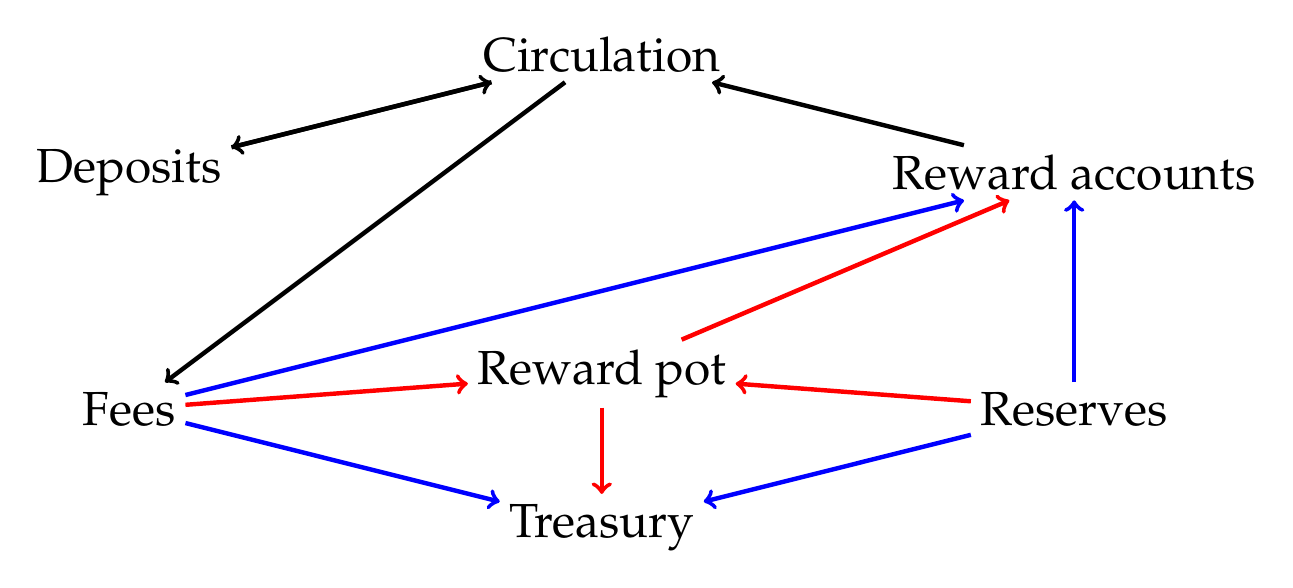
\begin{tikzpicture}
      [ x=30mm, y=30mm
      , direct/.style={black, draw}
      , implied/.style={blue, draw}
      , toTotPot/.style={red, draw}
      ]
    \node (C) at (3,2.5) {\LARGE Circulation};
    \node (R) at (5, 1) {\LARGE Reserves};
    \node (D) at (1, 2) {\LARGE Deposits};
    \node (FR) at (1,1) {\LARGE Fees};
    \node (RA) at (5, 2) {\LARGE Reward accounts};
    \node (T) at (3,0.5) {\LARGE Treasury};

    \draw[->, direct, ultra thick]
    (C) edge (D)
    (C) edge (FR)

    (D) edge (C)

    (RA) edge (C);

    \draw[->, implied, ultra thick]
    (FR) edge (T)
    (FR) edge (RA)

    (R) edge (T)
    (R) edge (RA);

    \node (TP) at (3, 1.15) {\LARGE Reward pot};

    \draw[->, toTotPot, ultra thick]
    (FR) edge (TP)
    (R) edge (TP)

    (TP) edge (RA)
    (TP) edge (T);
    \end{tikzpicture}
  \end{center}
  \caption{Preservation of Value}
  \label{fig:fund-preservation}
\end{figure}

Figure~\ref{fig:defs:reward-update} defines a reward update.
It consists of four pots:
\begin{itemize}
  \item The change to the treasury. This will be a positive value.
  \item The change to the reserves. This will be a negative value.
  \item The map of new individual rewards (to be added to the existing rewards).
  \item The change to the fee pot. This will be a negative value.
    rewards.
\end{itemize}

%%
%% Figure - Reward Update Defs
%%
\begin{figure}[htb]
  \emph{Reward Update}
  \begin{equation*}
    \RewardUpdate =
    \left(
      \begin{array}{r@{~\in~}ll}
        \Delta t & \Coin & \text{change to the treasury} \\
        \Delta r & \Coin & \text{change to the reserves} \\
        \var{rs} & \AddrRWD\mapsto\Coin & \text{new individual rewards} \\
        \Delta f & \Coin & \text{change to the fee pot} \\
      \end{array}
    \right)
  \end{equation*}
  %
  \caption{Rewards Update type}
  \label{fig:defs:reward-update}
\end{figure}

\clearpage

Figure~\ref{fig:functions:reward-update-creation} defines two functions,
$\fun{createRUpd}$ to create a reward update and $\fun{applyRUpd}$ to apply a
reward update to an instance of $\EpochState$.

The $\fun{createRUpd}$ function does the following:
\begin{itemize}
  \item Note that for all the calculations below, we use the previous protocol parameters
    $\var{prevPp}$, which corresponds to the parameters during the epoch for which we
    are creating rewards.
  \item First we calculate the change to the reserves,
    as determined by the $\rho$ protocol parameter.
  \item Next we calculate $\var{rewardPot}$, the total amount of coin available for rewards this
    epoch, as described in section 6.4 of \cite{delegation_design}. It consists of:
    \begin{itemize}
      \item The fee pot, containing the transaction fees from the epoch.
      \item The amount of monetary expansion from the reserves, calculated above.
    \end{itemize}
    Note that the fee pot is taken from the snapshot taken at the epoch boundary.
    (See~Figure\ref{fig:rules:snapshot}).
  \item Next we calculate the proportion of the reward pot that will move to the treasury,
    as determined by the $\tau$ protocol parameter. The remaining pot is called the
    $\var{R}$, just as in section 6.5 of \cite{delegation_design}.
  \item The rewards are calculated, using the oldest stake distribution snapshot (the one
    labeled ``go'').
    As given by $\fun{maxPool}$, each pool can receive a maximal amount, determined by its
    performance.  The difference between the maximal amount and the actual amount received is
    added to the amount moved to the treasury.
  \item The fee pot will be reduced by $\var{feeSS}$.
\end{itemize}

Note that fees are not explicitly removed from any account:
the fees come from transactions paying them and are accounted for whenever
transactions are processed.

The $\fun{applyRUpd}$ function does the following:
    \begin{itemize}
      \item Adjust the treasury, reserves and fee pots by the appropriate amounts.
      \item Add each individual reward to the global reward mapping.
        We must be careful, though, not to give out rewards to accounts
        that have been deregistered after the reward update was created.
        \begin{itemize}
          \item Rewards for accounts that are still registered are added to the reward mappings.
          \item The sum of the unregistered rewards are added to the reserves.
            % TODO - We may want to add these to the treasury instead, to be consistent with our other choices.
        \end{itemize}
    \end{itemize}

These two functions will be used in the blockchain transition systems in Section~\ref{sec:chain}.
In particular,
$\fun{createRUpd}$ will be used in Equation~\ref{eq:reward-update},
and $\fun{applyRUpd}$ will be used in Equation~\ref{eq:new-epoch}.

%%
%% Figure - The Reward Update Creation
%%
\begin{figure}[htb]
  \emph{Calculation to create a reward update}
  %
  \begin{align*}
    & \fun{createRUpd} \in \N \to \BlocksMade \to \EpochState \to \Coin \to \RewardUpdate \\
    & \createRUpd{slotsPerEpoch}{b}{es}{total} = \left(
      \Delta t_1,-~\Delta r_1+\Delta r_2,~\var{rs},~-\var{feeSS}\right) \\
    & ~~~\where \\
    & ~~~~~~~(\var{acnt},~\var{ss},~\var{ls},~\var{prevPp},~\wcard) = \var{es} \\
    & ~~~~~~~(\wcard,~\wcard,~\var{pstake_{go}},~\var{poolsSS},~\var{feeSS}) = \var{ss}\\
    & ~~~~~~~(\var{stake},~\var{delegs}) = \var{pstate_{go}} \\
    & ~~~~~~~(\wcard,~\var{reserves}) = \var{acnt} \\
    & ~~~~~~~\left(
      \wcard,~
      \left(
      \left(\var{rewards},~\wcard,~\wcard,~\wcard,~\wcard,~\wcard\right),~
      \wcard
      \right)
      \right) = \var{ls} \\
    & ~~~~~~~\Delta r_1 = \floor*{\min(1,\eta) \cdot (\fun{rho}~\var{prevPp}) \cdot
      \var{reserves}}
    \\
    & ~~~~~~~\eta =
      \begin{cases}
        1 & (\fun{d}~\var{prevPp})\geq 0.8 \\
        \frac{blocksMade}{\floor{(1-\fun{d}~\var{prevPp})\cdot\var{slotsPerEpoch} \cdot \ActiveSlotCoeff}}
          & \text{otherwise} \\
      \end{cases} \\
    & ~~~~~~~\var{rewardPot} = \var{feeSS} + \Delta r_1 \\
    & ~~~~~~~\Delta t_1 = \floor*{(\fun{tau}~\var{prevPp}) \cdot \var{rewardPot}} \\
    & ~~~~~~~\var{R} = \var{rewardPot} - \Delta t_1 \\
    & ~~~~~~~\var{circulation} = \var{total} - \var{reserves} \\
    & ~~~~~~~\var{rs}
      = \reward{prevPp}{b}{R}{(\dom{rewards})}{poolsSS}{stake}{delegs}{circulation} \\
    & ~~~~~~~\Delta r_{2} = R - \left(\sum\limits_{\_\mapsto c\in\var{rs}}c\right) \\
    & ~~~~~~~blocksMade = \sum_{\wcard \mapsto m \in b}m
  \end{align*}

  \caption{Reward Update Creation}
  \label{fig:functions:reward-update-creation}
\end{figure}

\begin{figure}[htb]
  \emph{Applying a reward update}
  %
  \begin{align*}
      & \fun{applyRUpd} \in \RewardUpdate \to \EpochState \to \EpochState \\
      & \fun{applyRUpd}~
      \left(
        \begin{array}{c}
          \Delta t \\
          \Delta r \\
          \var{rs} \\
          \Delta f \\
        \end{array}
    \right)
      \left(
        \begin{array}{c}
          \var{treasury} \\
          \var{reserves} \\
          ~ \\
          \var{rewards} \\
          \var{delegations} \\
          \var{ptrs} \\
          \var{genDelegs} \\
          \var{fGenDelegs} \\
          \var{i_{rwd}}
          \\~ \\
          \var{poolParams} \\
          \var{fPoolParams} \\
          \var{retiring} \\
          ~ \\
          \var{utxo} \\
          \var{deposited} \\
          \var{fees} \\
          \var{up} \\
          ~ \\
          \var{prevPp} \\
          \var{pp} \\
        \end{array}
      \right)
      =
      \left(
        \begin{array}{c}
          \varUpdate{\var{treasury} + \Delta t + \var{unregRU'}}\\
          \varUpdate{\var{reserves} + \Delta r}\\
          ~ \\
          \varUpdate{\var{rewards}\unionoverridePlus\var{regRU}} \\
          \var{delegations} \\
          \var{ptrs} \\
          \var{genDelegs} \\
          \var{fGenDelegs} \\
          \var{i_{rwd}}
          \\~ \\
          \var{poolParams} \\
          \var{fPoolParams} \\
          \var{retiring} \\
          ~ \\
          \var{utxo} \\
          \var{deposited} \\
          \varUpdate{\var{fees}+\Delta f} \\
          \var{up} \\
          ~ \\
          \var{prevPp} \\
          \var{pp} \\
        \end{array}
    \right) \\
    & ~~~\where \\
    & ~~~~~~~\var{regRU}=(\dom{rewards})\restrictdom rs\\
    & ~~~~~~~\var{unregRU}=(\dom{rewards})\subtractdom rs\\
    & ~~~~~~~\var{unregRU'}=\sum\limits_{\wcard\mapsto c\in\var{unregRU}} \var{c}\\
  \end{align*}

  \caption{Reward Update Application}
  \label{fig:functions:reward-update-application}
\end{figure}

\clearpage


\section{Blockchain layer}
\label{sec:chain}

\newcommand{\Proof}{\type{Proof}}
\newcommand{\Seedl}{\mathsf{Seed}_\ell}
\newcommand{\Seede}{\mathsf{Seed}_\eta}
\newcommand{\activeSlotCoeff}[1]{\fun{activeSlotCoeff}~ \var{#1}}
\newcommand{\slotToSeed}[1]{\fun{slotToSeed}~ \var{#1}}

\newcommand{\T}{\type{T}}
\newcommand{\vrf}[3]{\fun{vrf}_{#1} ~ #2 ~ #3}
\newcommand{\verifyVrf}[4]{\fun{verifyVrf}_{#1} ~ #2 ~ #3 ~#4}

\newcommand{\HashHeader}{\type{HashHeader}}
\newcommand{\HashBBody}{\type{HashBBody}}
\newcommand{\bhHash}[1]{\fun{bhHash}~ \var{#1}}
\newcommand{\bHeaderSize}[1]{\fun{bHeaderSize}~ \var{#1}}
\newcommand{\bSize}[1]{\fun{bSize}~ \var{#1}}
\newcommand{\bBodySize}[1]{\fun{bBodySize}~ \var{#1}}
\newcommand{\OCert}{\type{OCert}}
\newcommand{\BHeader}{\type{BHeader}}
\newcommand{\BHBody}{\type{BHBody}}

\newcommand{\bheader}[1]{\fun{bheader}~\var{#1}}
\newcommand{\hsig}[1]{\fun{hsig}~\var{#1}}
\newcommand{\bprev}[1]{\fun{bprev}~\var{#1}}
\newcommand{\bhash}[1]{\fun{bhash}~\var{#1}}
\newcommand{\bvkcold}[1]{\fun{bvkcold}~\var{#1}}
\newcommand{\bseedl}[1]{\fun{bseed}_{\ell}~\var{#1}}
\newcommand{\bprfn}[1]{\fun{bprf}_{n}~\var{#1}}
\newcommand{\bseedn}[1]{\fun{bseed}_{n}~\var{#1}}
\newcommand{\bprfl}[1]{\fun{bprf}_{\ell}~\var{#1}}
\newcommand{\bocert}[1]{\fun{bocert}~\var{#1}}
\newcommand{\bnonce}[1]{\fun{bnonce}~\var{#1}}
\newcommand{\bleader}[1]{\fun{bleader}~\var{#1}}
\newcommand{\hBbsize}[1]{\fun{hBbsize}~\var{#1}}
\newcommand{\bbodyhash}[1]{\fun{bbodyhash}~\var{#1}}
\newcommand{\overlaySchedule}[4]{\fun{overlaySchedule}~\var{#1}~\var{#2}~{#3}~\var{#4}}

\newcommand{\PrtclState}{\type{PrtclState}}
\newcommand{\PrtclEnv}{\type{PrtclEnv}}
\newcommand{\OverlayEnv}{\type{OverlayEnv}}
\newcommand{\VRFState}{\type{VRFState}}
\newcommand{\NewEpochEnv}{\type{NewEpochEnv}}
\newcommand{\NewEpochState}{\type{NewEpochState}}
\newcommand{\PoolDistr}{\type{PoolDistr}}
\newcommand{\BBodyEnv}{\type{BBodyEnv}}
\newcommand{\BBodyState}{\type{BBodyState}}
\newcommand{\RUpdEnv}{\type{RUpdEnv}}
\newcommand{\ChainEnv}{\type{ChainEnv}}
\newcommand{\ChainState}{\type{ChainState}}
\newcommand{\ChainSig}{\type{ChainSig}}

In Figure~\ref{fig:functions:to-ma}, we give the functions that will be used
to transition from a Sophie chain state into a chain state that provides multi-asset support.
The only part of the state that is affected by the transition is the UTxO. For ease of
reading, we keep the function $\fun{updateChainStateUTxO}$ abstract, which simply transforms the
UTxO that is nested deeply inside the chain state with the provided function.

%%
%% Figure - Sophie to MA Transition
%%
\begin{figure}[htb]
  %
  \emph{Abstract function}
  %
  \begin{align*}
      & \fun{updateChainStateUTxO} \in (\SophieUTxO \to \UTxO) \to \SophieChainState \to \ChainState \\
      & \text{update the UTxO in a Sophie chain state}
  \end{align*}
  %
  \emph{Chain state update}
  %
  \begin{align*}
      & \fun{mkUTxO} ~\in~ \SophieUTxO  \to \UTxO  \\
      & \fun{mkUTxO}~\var{utxo} ~=~ \{~ \var{txin} \mapsto (a,\fun{inject}~c) ~\vert~
      \var{txin} \mapsto \var{(a,c)}\in ~\var{utxo}~\}
      \nextdef
      & \fun{toMA} \in ~ \SophieChainState \to \ChainState \\
      & \fun{toMA}~cs = \fun{updateChainStateUTxO}~\fun{mkUTxO}
  \end{align*}
  \caption{Sophie to Multi-Asset Chain State Transtition}
  \label{fig:functions:to-ma}
\end{figure}

\section{Transition Systems Properties}
\label{sec:ts-properties}


\subsection{Transition-system traces}
\label{sec:ts-traces}

This section introduces the notion of traces induced by the transition systems
described in \cite{small_step_semantics}.

\begin{definition}[Traces]
  Given a state transition system $L=(S,T,\Sigma, R, \Gamma)$, the set of
  traces of $L$, denoted as $\fun{traces}_L$ is defined as:
  $$
  \{ (e, s, \txs, s') \mid e \in \Gamma,~ s \in S,~ \txs \in \seqof{\Sigma},~ s' \in S\}
  $$

\end{definition}


\begin{definition}[Valid traces]
  Given a state transition system $L=(S,T,\Sigma, R, \Gamma)$, we define the
  notion of valid traces inductively:

  \begin{itemize}
  \item For all $e \in \Gamma$, $s \in S$, $(e, s, \epsilon, s)$ is a valid
    trace of $L$.

  \item If $(e, s, \txs, s')$ is a valid trace, and
    $e \vdash s' \trans{}{\var{t}} s''$ is a valid transition according to the
    rules of $L$, then $(e, s, \txs; t, s'')$ is also a valid trace.
  \end{itemize}

\end{definition}

We denote the set of valid traces of $L$ as $\transtar{L}{}$, and we write
$e \vdash s \transtar{L}{\txs} s'$ as a shorthand for
$(e, s, \txs, s') \in \transtar{L}{}$. Furthermore, when the transition system
name is clear from the context we will omit it from the transition arrow label.

\subsection{Additional notation}
\label{sec:additional-notation}

We describe next additional notation needed in the properties of the transition
systems specified in this document.

\subsubsection{Sequence indexing}
\label{sec:seq-indexing}

Given a sequence $\mathcal{A} \in \seqof{\type{A}}$, and a natural number $i$
such that $0 \leq i < \size{\mathcal{A}}$, $\mathcal{A}_i$ refers to the
$i^{\text{th}}$ element of $\mathcal{A}$.


Given a sequence $\mathcal{A}$, a quantification symbol $\bigoplus$, e.g.
$\forall$ or $\exists$, a range predicate $R$, and a quantification term $T$
(both of which depend on an element of $\mathcal{A}$) we write:
%
$$
\bigoplus \mathcal{A}_i \cdot R~\mathcal{A}_i \cdot T~\mathcal{A}_i
$$
%
as a shorthand notation for:
%
$$
\bigoplus i \cdot 0 \leq i < \size{\mathcal{A}} \wedge R~\mathcal{A}_i \cdot T~\mathcal{A}_i
$$

For instance:
%
$$
\forall \txs_i \cdot \txins{\txs_i} \neq \emptyset
$$
is a shorthand notation for:
$$
\forall i \cdot 0 \leq i < \size{\txs} \Rightarrow \txins{\txs_i} \neq \emptyset
$$
Remember that the range of a universal quantification can be expressed by an
implication, and the range of an existential qualification by a conjunction.

\subsubsection{Quantifying over set operations}
\label{sec:quantifying-over-set-operators}

Given a sequence $\mathcal{A} \in \seqof{A}$, a set $B$, a set operation
$\bigoplus$, e.g. $\cup$ or $\unionoverrideRight$, and a function
$\fun{f} \in \type{A} \to \type{B}$, the term:
%
$$
\underset{\fun{f}}{\bigoplus} \mathcal{A}
$$
is a shorthand notation for:
%
$$
\underset{0 \leq i < \size{\mathcal{A}}}{\bigoplus} \mathcal{A}_i
$$

For instance:
$$
\bigcup_{\txins{}} \txs
$$
denotes the sequence of unions:
$$
\bigcup_{0 \leq i < \size{\txs}} \txins{\txs_i}
$$

In a set operation quantification over a sequence $\mathcal{A}$, the operation
is applied to the elements the order in which they appear in $\mathcal{A}$.
This is crucial in the case of non-commutative operations, such as union
override ($\unionoverrideRight$).

\subsection{UTxO Properties}
\label{sec:utxo-properties}

Property~\ref{prop:no-double-spending} expresses the fact that transaction
inputs cannot be used more than once. This property requires that the starting
UTxO does not contain any future outputs, which is a reasonable constraint.

\begin{property}[No double spending]\label{prop:no-double-spending}
  For all

  $$
  \left(
    \begin{array}{l}
      \var{utxo_0}\\
      \var{reserves_0}
    \end{array}
  \right)
  \transtar{\hyperref[fig:rules:utxo]{utxo}}{\txs}
  \left(
    \begin{array}{l}
      \var{utxo}\\
      \var{reserves}
    \end{array}
  \right)
  $$

  such that

  $$
    \forall \txs_i \cdot \dom~(\txouts{\txs_i}) \cap \dom~(\var{utxo_0}) = \emptyset
  $$

  we have:

  $$
  \forall \txs_i,~\txs_j \cdot i < j \Rightarrow \txins{\txs_i} \cap \txins{\txs_j} = \emptyset
  $$
\end{property}

Property~\ref{prop:utxo-out-min-in} expresses the fact that all inputs and
outputs are accounted for, in such a way that we can reconstruct the final
(UTxO) state by adding all the outputs to the initial state, and removing the
spent outputs.

\begin{property}[UTxO is outputs minus inputs]\label{prop:utxo-out-min-in}
  For all

  $$
  \left(
    \begin{array}{l}
      \var{utxo_0}\\
      \var{reserves_0}
    \end{array}
  \right)
  \transtar{\hyperref[fig:rules:utxo]{utxo}}{\txs}
  \left(
    \begin{array}{l}
      \var{utxo}\\
      \var{reserves}
    \end{array}
  \right)
  $$

  such that

  $$
    \forall \txs_i \cdot \dom~(\txouts{\txs_i}) \cap \dom~(\var{utxo_0}) = \emptyset
  $$

  we have:

  $$
  \bigcup_{\txins{}} \txs \subtractdom (\var{utxo_0} \cup \bigcup_{\txouts{}} \txs) = \var{utxo}
  $$

\end{property}

Property~\ref{prop:utxo-money-supply-cnst} models the fact that the amount of
money in the system (counted as Entropics) remains constant.

\begin{property}[Money supply is constant in the system]\label{prop:utxo-money-supply-cnst}
  For all

  $$
  \left(
    \begin{array}{l}
      \var{utxo_0}\\
      \var{reserves_0}
    \end{array}
  \right)
  \transtar{\hyperref[fig:rules:utxo]{utxo}}{\txs}
  \left(
    \begin{array}{l}
      \var{utxo}\\
      \var{reserves}
    \end{array}
  \right)
  $$

  we have:

  $$ \var{reserves} + \balance{utxo} =  \var{reserves_0} + \balance{utxo_0} $$
\end{property}

\subsection{Delegation Properties}
\label{sec:delegation-props}

Property~\ref{prop:no-dcert-replay} states that delegation certificates cannot be replayed. Remember
that $\Delta_i$ is the $i^{\text{th}}$ element of $\Delta$, which is a sequence of sequences of
delegation certificates, so $\Delta_i \in \seqof{\DCert}$ and $\Delta_{i_j} \in \DCert$ (assuming
$j$ is a valid index of $\Delta_i$).

\begin{property}[No replay of delegation certificates]\label{prop:no-dcert-replay}
  For all
  %
  $$
  \left(
    \begin{array}{l}
      \var{delegSt}
    \end{array}
  \right)
  \transtar{\hyperref[fig:rules:delegation-interface]{deleg}}{\Delta}
  \left(
    \begin{array}{l}
      \var{delegSt'}
    \end{array}
  \right)
  $$
  %
  we have:
  %
  $$
  \forall i, j, k, l \cdot j < l \Rightarrow \Delta_{i_j} \neq \Delta_{k_l}
  $$
\end{property}



\addcontentsline{toc}{section}{References}
\bibliographystyle{plainnat}
\bibliography{references}

\begin{appendix}
  \section{Script Constructors and Evaluation}
\label{sec:timelock-lang}


\begin{figure}[htb]
  \begin{align*}
    \fun{validateScript} & \in\Script\to\Tx\to\Bool \\
    \fun{validateScript} ~s~\var{tx}~& =~
                             \fun{evalTimelock}~\var{vhks} ~\var{itr}~\var{s} \\
                         & ~~~~\where \\
                         & ~~~~~~~~\var{vhks}\leteq \{\fun{hashKey}~vk \vert
                           vk \in \dom(\fun{txwitsVKey}~\var{tx})\} \\
                         & ~~~~~~~~\var{itr} \leteq \fun{txvldt}~ (\txbody~ \var{tx})
  \end{align*}
  \caption{Script Validation}
  \label{fig:functions-validate}
\end{figure}

In the SophieMA era, the
$\fun{validateScript}$ function performs validation of only timelock scripts,
see Figure~\ref{fig:functions-validate}. Note that while there is no explicit
support for validating multi-signature scripts in $\fun{validateScript}$,
these scripts remain effectively usable as the encodings of multi-sig and timelock
scripts are compatible. An existing multi-sig script-locked output is
spent by interpreting the encoded script as a timelock script (one without
any validity interval clauses), then validating it. For details, see the CDDL
specification.

The arguments that are passed to the $\fun{validateScript}$ function include all those
that are needed for $\Timelock$ script evaluation :

\begin{itemize}
\item The script getting evaluated
\item The transaction
\end{itemize}

The semantics of the Timelock language are specified in Figure~\ref{fig:defs:tx-mc-eval}.
The evaluation of the scripts constructed by $\type{Signature}, \type{AllOf},
\type{AnyOf}, \type{MOfN}$ is done the same as for their
$\ScriptNI$ counterparts. The $\type{RequireTimeStart}$ evaluation
checks that the start of the transaction validity interval is not $\Nothing$, and is in or after
the slot specified by the constructor. The $\type{RequireTimeExpire}$ evaluation
checks that the end of the transaction validity interval is not $\Nothing$, and is in or before
the slot specified by the constructor.

\begin{figure*}[htb]
  \emph{Timelock Script Constructor Types}
  \begin{align*}
    & \type{evalTimelock} & \in \powerset{\KeyHash}\to(\Slot^? \times \Slot^?)\to\Timelock \to \Bool & \\
    & \text{The type of the Timelock script evaluator} \\~\\
    %
    & \type{Signature} & \in \KeyHash \to \Timelock & \\
    %
    & \type{AllOf} & \in \seqof{\Timelock} \to \Timelock & \\
    %
    & \type{AnyOf} & \in \seqof{\Timelock} \to \Timelock & \\
    %
    & \type{MOfN} & \in \N \to \seqof{\Timelock} \to \Timelock & \\
    %
    & \type{RequireTimeStart} & \in \Slot \to \Timelock &\\
    %
    & \type{RequireTimeExpire} & \in \Slot \to \Timelock &\\
  \end{align*}
  %
  \emph{Timelock Script Evaluation}
  \begin{align*}
    \fun{evalTimelock} & ~(\type{Signature}~hk)~\var{vhks}~\wcard =  hk \in vhks \\
    \fun{evalTimelock} & ~(\type{AllOf}~ts)~\var{vhks}~\wcard =
                              \forall t \in ts: \fun{evalTimelock}~t~vhks\\
    \fun{evalTimelock} & ~(\type{AnyOf}~ts)~\var{vhks}~\wcard =
                              \exists t \in ts: \fun{evalTimelock}~t~vhks\\
    \fun{evalTimelock} & ~(\type{MOfN}~m~ts)~\var{vhks}~\wcard = \\
                             & m \leq \Sigma
                               (\textrm{card} \{ t s.t. t \leftarrow ts \wedge \fun{evalTimelock}~\var{t}~\var{vhks} \\
    \fun{evalTimelock} &~(\type{RequireTimeStart}~\var{lockStart})~\var{vhks}~\var{(\var{txStart}, \wcard)} \\
    & =~
    \begin{cases}
      \False & \var{txStart} = \Nothing \\
      \var{lockStart} \leq \var{txStart} & \text{otherwise}
    \end{cases} \\
    \fun{evalTimelock} &~(\type{RequireTimeExpire}~\var{lockExp})~\var{vhks}~\var{(\wcard, \var{txExp})} \\
    & =~
    \begin{cases}
      \False & \var{txExp} = \Nothing \\
      \var{txExp} \leq \var{lockExp} & \text{otherwise}
    \end{cases} \\
  \end{align*}
  \caption{Timelock Script Constructor Types and Evaluation}
  \label{fig:defs:tx-mc-eval}
\end{figure*}

% The Figures~\ref{fig:defs:tx-mc-eval},~\ref{fig:defs:tx-mc-eval-2},
% and~\ref{fig:whitelist-example} give
% possible constructors of the Timelock language.
%
% %% \begin{note}
% %%   sort out the constructors
% %% \end{note}
%
% \begin{figure*}[htb]
%   \begin{align*}
%     & \fun{evalTimelock} \in\Timelock\to\PolicyID\to\Slot\to\powerset\KeyHash \\
%     &~~~~\to\TxBody\to\UTxO \to\Bool  \\
%     & \text{UTxO is only for the outputs THIS tx is spending, not global UTxO, i.e.} \\
%     & \text{when called,}~\var{spentouts}~=~(\fun{txins}~\var{txb}) ~\restrictdom~\var{utxo} \\~\\
%     %
%     & \fun{evalTimelock}  ~(\type{JustMSig}~s)~\var{pid}~\var{slot}~\var{vhks}
%      ~\var{txb}~\var{spentouts} \\
%     &~~~~ =~ \fun{evalMultiSigScript}~s~\var{vhks} \\
%     & \text {checks the msig script}\\~\\
%     %
%     & \fun{evalTimelock}
%      ~\type{DoMint}~\var{pid}~ \var{slot}~\var{vhks} ~\var{txb}~\var{spentouts} \\
%     &~~~~ =~ \var{pid} \notin \dom~(\fun{mint}~\var{txb}) \\
%     & \text {checks that script hash of this script is not an asset ID being minted by tx}  \\~\\
%     %
%     & \fun{evalTimelock}
%      ~\type{SignedByPIDToken}~\var{pid}~ \var{slot}~\var{vhks} ~\var{txb}~\var{spentouts} \\
%     &~~~~ =~ \exists~t\mapsto ~\_~\in~ \fun{range}~(\var{pid}~ \restrictdom~(\fun{ubalance}~\var{spentouts})) ~:~ t~\in~\var{vhks} \\
%     & \text{checks that tx is signed by a key whose hash is the name of a token in this asset}
%     \\~\\
%     & \fun{evalTimelock}
%      ~(\type{SpendsCur}~\var{pid'})~\var{pid}~ \var{slot}~\var{vhks} ~\var{txb}~\var{spentouts} \\
%     &~~~~ =~ (\var{pid'}~\neq~\Nothing ~\wedge ~\var{pid'}~\in~ \dom~(\fun{ubalance}~\var{spentouts}))\\
%     &~~~~~~ \vee (\var{pid'}~=~\Nothing ~\wedge ~\var{pid}~\in~ \dom~(\fun{ubalance}~\var{spentouts})) \\
%     & \text{checks that this transaction spends asset pid' OR itself if}~\var{pid'}~=~\Nothing
%     \\~\\
%     &\fun{evalTimelock}~(\type{Not}~s)~\var{pid}~\var{slot}~\var{vhks}
%     ~\var{txb}~\var{spentouts}
%    \\
%     &~~~~ = \neg ~\fun{evalTimelock}~s~\var{pid}~\var{slot}~\var{vhks}
%     ~\var{txb}~\var{spentouts}\\~\\
%     %
%     &\fun{evalTimelock}~(\type{RequireAll}~ls)~\var{pid}~\var{slot}~\var{vhks}
%     ~\var{txb}~\var{spentouts}
%    \\
%     &~~~~ = \forall ~s'~ \in~ ls~:~\fun{evalTimelock}~s'~\var{pid}~\var{slot}~\var{vhks}
%     ~\var{txb}~\var{spentouts}\\~\\
%     %
%     &\fun{evalTimelock}~(\type{RequireOr}~ls)~\var{pid}~\var{slot}~\var{vhks}
%     ~\var{txb}~\var{spentouts}
%    \\
%     &~~~~ = \exists ~s'~ \in~ ls~:~\fun{evalTimelock}~s'~\var{pid}~\var{slot}~\var{vhks}
%     ~\var{txb}~\var{spentouts}\\
%   \end{align*}
%   \caption{Multi-asset Script Evaluation}
%   \label{fig:defs:tx-mc-eval}
% \end{figure*}
%
% \begin{figure*}[htb]
%   \begin{align*}
%     & \fun{evalTimelock}
%      ~(\type{AssetToAddress}~\var{pid'}~\var{addr})~\var{pid}~ \var{slot}~\var{vhks} ~\var{txb}~\var{spentouts} \\
%     &~~~~ =~ \forall~(a, v)~\in~\fun{range}~(\fun{outs}~txb),~\\
%     &~~~~~~ \var{c}~\in~\dom~v~\Rightarrow~(a~=~ \var{a'} ~\wedge~
%                        v~=~\var{c}~ \restrictdom~(\fun{ubalance}~(\fun{outs}~txb)) \\
%     & \where \\
%     & ~~~~~~~ \var{a'}~=~\fun{if}~ \var{addr}~\neq~\Nothing~\fun{then}~\var{addr}~\fun{else}~\var{(pid',pid')} \\
%     & ~~~~~~~ \var{c}~=~\fun{if}~ \var{pid'}~\neq~\Nothing~\fun{then}~\var{pid'}~\fun{else}~\var{pid} \\
%     & \text{checks that tx outputs any pid tokens by themselves to the specified address} \\
%     & \text {the script address of the given asset when addr unspecified} \\~\\
%     & \fun{evalTimelock}
%      ~(\type{TrancheTokens}~\var{tts}~\var{txin})~\var{pid}~\var{slot}~\var{vhks}
%      ~\var{txb}~\var{spentouts}  \\
%     &~~~~ =~(\var{pid}\mapsto\var{tts}~\in~\var{val})~ \wedge~(\var{txin}~\in~\fun{txins}~{txb}) \\
%     & \text{tranche tokens is incomplete} \\~\\
%     %
%     & \fun{evalTimelock}
%      ~(\type{FreshTokens})~\var{pid}~\var{slot}~\var{vhks}
%      ~\var{txb}~\var{spentouts}
%       \\
%     &~~~~ =~\forall~\var{pid}~ \mapsto ~tkns ~\in~ \var{val}~:~ \\
%     &~~~~ \forall~t~\in~\var{tkns},~
%         \fun{nameToken}~(\fun{indexof}~\var{t}~\var{tkns},~\fun{txins}~{txb})~=~t
%     \end{align*}
%     \caption{Multi-asset Script Evaluation, cont.}
%     \label{fig:defs:tx-mc-eval-2}
% \end{figure*}
%
% \begin{figure*}[htb]
%   \begin{align*}
%     & \fun{whitelist} \in\ScriptMSig\to\Script  \\~\\
%     %
%     & \type{whitelist}  ~\var{msig}~ =~ \type{RequireOr}~
%       (\type{RequireAll}~(\type{DoMint};~\type{JustMSig}~\var{msig});~\\
%     &~~~~~~ \type{RequireAll}~(\type{AssetToAddress}~\Nothing~\Nothing ;\\
%     &~~~~~~ (\type{Not}~\type{DoMint});~\type{SignedByPIDToken})) \\
%     %
%     & \text{msig is some MSig script containing signatures of some accreditation authority} \\
%     & \text{i.e. this authority can do any minting or spending of this token} \\~\\
%     %
%     & (\fun{hashScript}~(\type{SpendsCur}~(\fun{hashScript}~(\type{whitelist}~\var{msig}))),~ \var{tkns}) \\
%     & \text{an example of an output spending which requires to be on a whitelist made by msig authority}
%   \end{align*}
%   \caption{Whitelist Script Example}
%   \label{fig:whitelist-example}
% \end{figure*}

  \section{Output Size}
\label{sec:value-size}

In Sophie, the protocol parameter $\var{minUTxOValue}$ is used to
disincentivize attacking nodes by putting many small outputs on the
UTxO, permanently blocking memory. Because members of the $\Value$
type can be arbitrary large, the ledger requires a $\UTxO$ entry to
contain a minimum amount of Bcc, proportional to its size.

There is also another $\Value$ size consideration with respect to spendability
of an output. The restriction on the total serialized size of the transaction (set
by the parameter $\var{maxTxSize}$) serves as an implicit upper bound on the
size of a $\Value$ contained in an output of a transaction. Without tighter
limits on the output $\Value$ size, one of the following situations could arise,
causing the output to be come unspendable (these are just a two examples) :

\begin{itemize}
  \item The script locking the very large $\Value$-containing UTxO is too large
  to fit inside the transaction alongside the $\Value$ itself while still respecting
  the max transaction size
  \item The large $\Value$ cannot be split into several outputs, because the
  outputs are impossible to fit inside a single transaction
\end{itemize}

Figure \ref{fig:size-helper} contains abstract and helper functions
used in calculating the in-memory and serialized representation
sizes of $\Value$ terms.

\begin{figure*}[h]
  \emph{Abstract Functions}
  %
  \begin{align*}
    & \fun{serSize} \in \Value \to \MemoryEstimate \\
    & \text{Gives the size of the serialized representation of a $\Value$}
    \nextdef
    & \fun{anameLen} \in \AssetName \to \MemoryEstimate \\
    & \text{Returns the length (in bytes) of an asset name}
  \end{align*}
  %
  \emph{Helper Functions}
  \begin{align*}
    & \fun{numAssets} \in \Value \to \N \\
    & \fun{numAssets}~{vl}~=~\|~\{~(pid, an)~\vert~pid~(\mapsto~(an~\mapsto~\wcard))~\in~vl~\}~\| \\
    & \text{Returns the number of distinct asset IDs in a $\Value$}
    & \nextdef
    & \fun{sumALs} \in \Value \to \N \\
    & \fun{sumALs}~{vl}~=~ \sum_{\{~an~\vert~\wcard~(\mapsto~(an~\mapsto~\wcard))~\in~vl~\}} \fun{anameLen}~an \\
    & \text{Returns the sum of the lengths (in bytes) of distinct asset names in a $\Value$}
    & \nextdef
    & \fun{numPids} \in \Value \to \N \\
    & \fun{numPids}~{vl} ~=~ \|~\supp~{vl}~\| \\
    & \text{The number of policy IDs in a $\Value$}
  \end{align*}
  \caption{Value Size}
  \label{fig:size-helper}
\end{figure*}

The function $\fun{serSize}$, unlike the functions $\fun{size}$ and $\fun{utxoEntrySize}$
    (explained below), is left abstract. It returns the actual number of bytes a $\Value$
    occupies in the serialized transaction (and hence is implementation-dependent).

    One reason for this design decision is that the $\fun{serSize}$ function is used constrain
    the serialized representation of the transaction (in particular, the size
    of $\Value$ terms in outputs), whereas the min-Bcc requirement is about
    the in-memory representation size. Moreover, a transparently-calculated size estimate
    is not necessary for limiting the size of values in outputs, since this size-bound
    check does not place any additional accounting/monetary constranits on transaction construction,
    unlike the min-Bcc requirement.

Figure \ref{fig:min-val-calc} gives the types of constants used in the estimation
of the size of a UTxO entry, and the associated min-Bcc-value.

\begin{figure*}[h]
  \emph{Constants}
  \begin{equation*}
    \begin{array}{lcl}
      (k_0, k_1, k_2, k_3, k_4) & \in & \N \times \N \times \N \times \N \times \N \\
      \mathsf{UtxoEntrySizeWithoutVal} & \in & \MemoryEstimate \\
      \mathsf{BccOnlyUTxOSize} & \in & \MemoryEstimate \\
      \mathsf{MaxValSize} & \in & \MemoryEstimate \\
    \end{array}
  \end{equation*}
  %
  \emph{Size and Min-Bcc Functions}
  \begin{align*}
    & \fun{size} \in \Value \to \MemoryEstimate \\
    & \fun{size}~\var{vl} ~=~
    \begin{cases}
      k_0 & \fun{bccOnly}~vl~=~vl \\
      k_1 + \lfloor~ (((\fun{numAssets}~vl) * k_2) + (\fun{sumALs}~vl) & \\
      ~~~~~~ + ((\fun{numPids}~vl) * k_3) + (k_4 - 1)))~ /~ k_4~\rfloor & \text{otherwise} \\
    \end{cases} \\
    & \text{Calculate the size of a $\Value$}
    \nextdef
    & \fun{bccPerUTxOWord}~\in \PParams \to \Coin \\
    & \fun{bccPerUTxOWord}~pp = \lfloor~ (\fun{minUTxOValue}~pp~/~ \mathsf{bccOnlyUTxOSize})~ \rfloor \\
    & \text{Calculate the cost of storing a memory unit of data as a UTxO entry}
    \nextdef
    & \fun{utxoEntrySize} \in \TxOut \to \MemoryEstimate \\
    & \fun{utxoEntrySize}~\var{out} = \mathsf{utxoEntrySizeWithoutVal} + \fun{size}~ (\fun{getValue}~out) \\
    & \text{Calculate the size of a UTxO entry}
\end{align*}
\caption{Value Size}
\label{fig:min-val-calc}
\end{figure*}

The $\fun{size}$ function returns the estimated size of a $\Value$ term. It is constant in the
case where the value contains only Bcc. If there are other types of tokens in the
term, the size depends on

\begin{itemize}
  \item the number of distinct asset types (asset IDs)
  \item the number of distinct policy IDs, and
  \item the sum of the lengths of distinct asset names of the tokens.
\end{itemize}

The parameter $\fun{minUTxOValue}$ specifies the min-Bcc value for a UTxO containing
only Bcc. This type of UTxO varies in size somewhat (eg. Cole style addresses
may be a different length than Sophie ones), but we estimate the size of the most commonly
used type of Bcc-only UTxO as the constant value $\mathsf{bccOnlyUTxOSize}$.
This constant is in fact an upper bound on UTxOs which have have only Sophie credentials.

We use this size estimate
to calculate what $\fun{minUTxOValue}$ implies to be the min-Bcc value requirement
\emph{per word} of UTxO data.

The function $\fun{bccPerUTxOWord}$ performs this calculation by dividing the
min-Bcc value by the Bcc-only UTxO size.

The $\mathsf{utxoEntrySizeWithoutVal}$ is the constant representing
the size of a UTxO entry, not counting the size of the $\Value$ term it contains.
Here, again, the actual size of a UTxO (excluding the $\Value$) can vary, but
we use an upper bound on the size of Sophie-credential UTxOs.

The function $\fun{utxoEntrySize}$ estimates the size of an arbitrary SophieMA-era
UTxO. It adds the size estimate of the $\Value$ term in a UTxO and the
$\mathsf{utxoEntrySizeWithoutVal}$ constant.

The constants used in the implementation of the Aurum era are as follows :

\begin{itemize}
  \item $(k_0, k_1, k_2, k_3, k_4) = (2, 6, 12, 28, 8)$
  \item $\mathsf{utxoEntrySizeWithoutVal} = 27$ words (8 bytes)
  \item $\mathsf{bccOnlyUTxOSize} = 27$ words (8 bytes)
  \item $\mathsf{MaxValSize} = 4000$ bytes, ie. 500 words.
\end{itemize}

\end{appendix}

\end{document}
